\section{Results and Discussion}
\label{ch4:sec:results-and-discussion}

In this section, all presented results were generated from the simulation of the different cases.
In each of the following three subsections, the performances of the AIMD and AIMD+ algorithm are compared against each other and the baseline cases.
To do so, the performance metrics that were outlined in Section~\ref{ch4:subsec:performance-metric-definition} are used.
Results from the four test cases, which have been defined as \ref{ch4:case-a}, \ref{ch4:case-b}, \ref{ch4:case-c} and \ref{ch4:case-d} in Section~\ref{ch4:subsec:test-cases-and-scenarios}, are explained first.
Then the results from the full analysis over the large range of EV and battery storage uptake is presented.

\subsection{Voltage Violation Analysis}

\begin{figure}\centering
	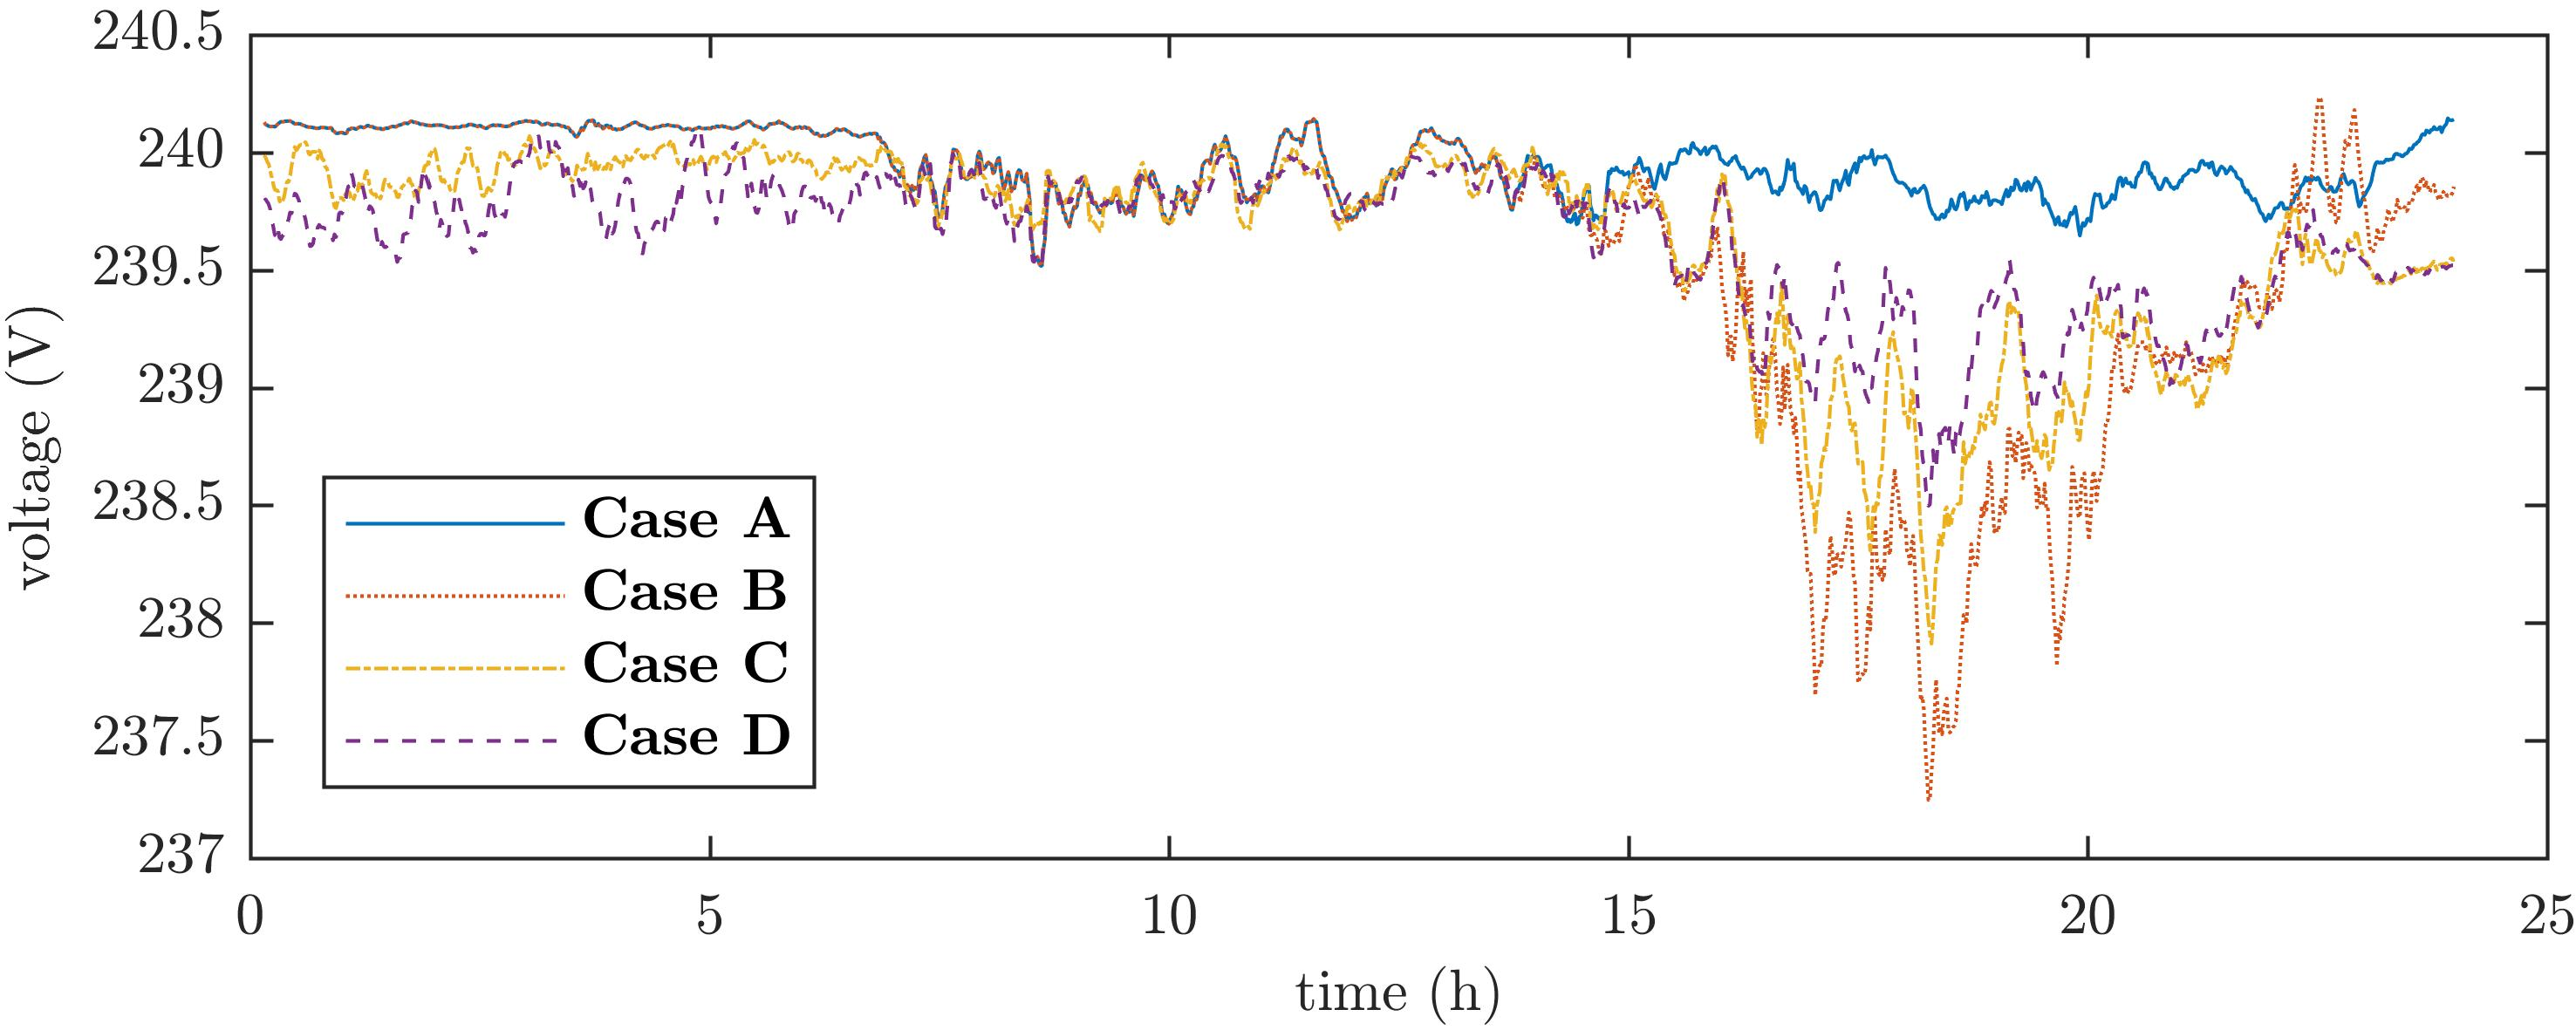
\includegraphics{_chapter4/fig/voltage-profiles}
	\caption{Mean voltage profiles for all four test cases over a single day.}
	\label{ch4:fig:voltage-profiles}
\end{figure}


For the assessment of improving voltage levels, results are compared for the algorithms' performances at reducing bus voltage deviation; particularly by increasing the lowest recorded bus voltage.
Each load's bus voltage was recorded, from which a sample voltage profile, Figure~\ref{ch4:fig:voltage-profiles}, was extracted, where the bus voltage fluctuation over time becomes apparent. It can be seen that the introduction of EVs has significantly lowered the line-to-neutral voltage. Adding energy BESS devices did raise the voltage levels during times of peak demand, as can be seen between 17:00 and 21:00, where the AIMD+ algorithm has elevated voltages further than the AIMD scenario. To obtain a better understanding of the level of improvement, the voltage frequency distribution of all buses along the feeder was generated and plotted in a histogram in Figure~\ref{ch4:fig:voltage-probabilities}.

\begin{figure}\centering
 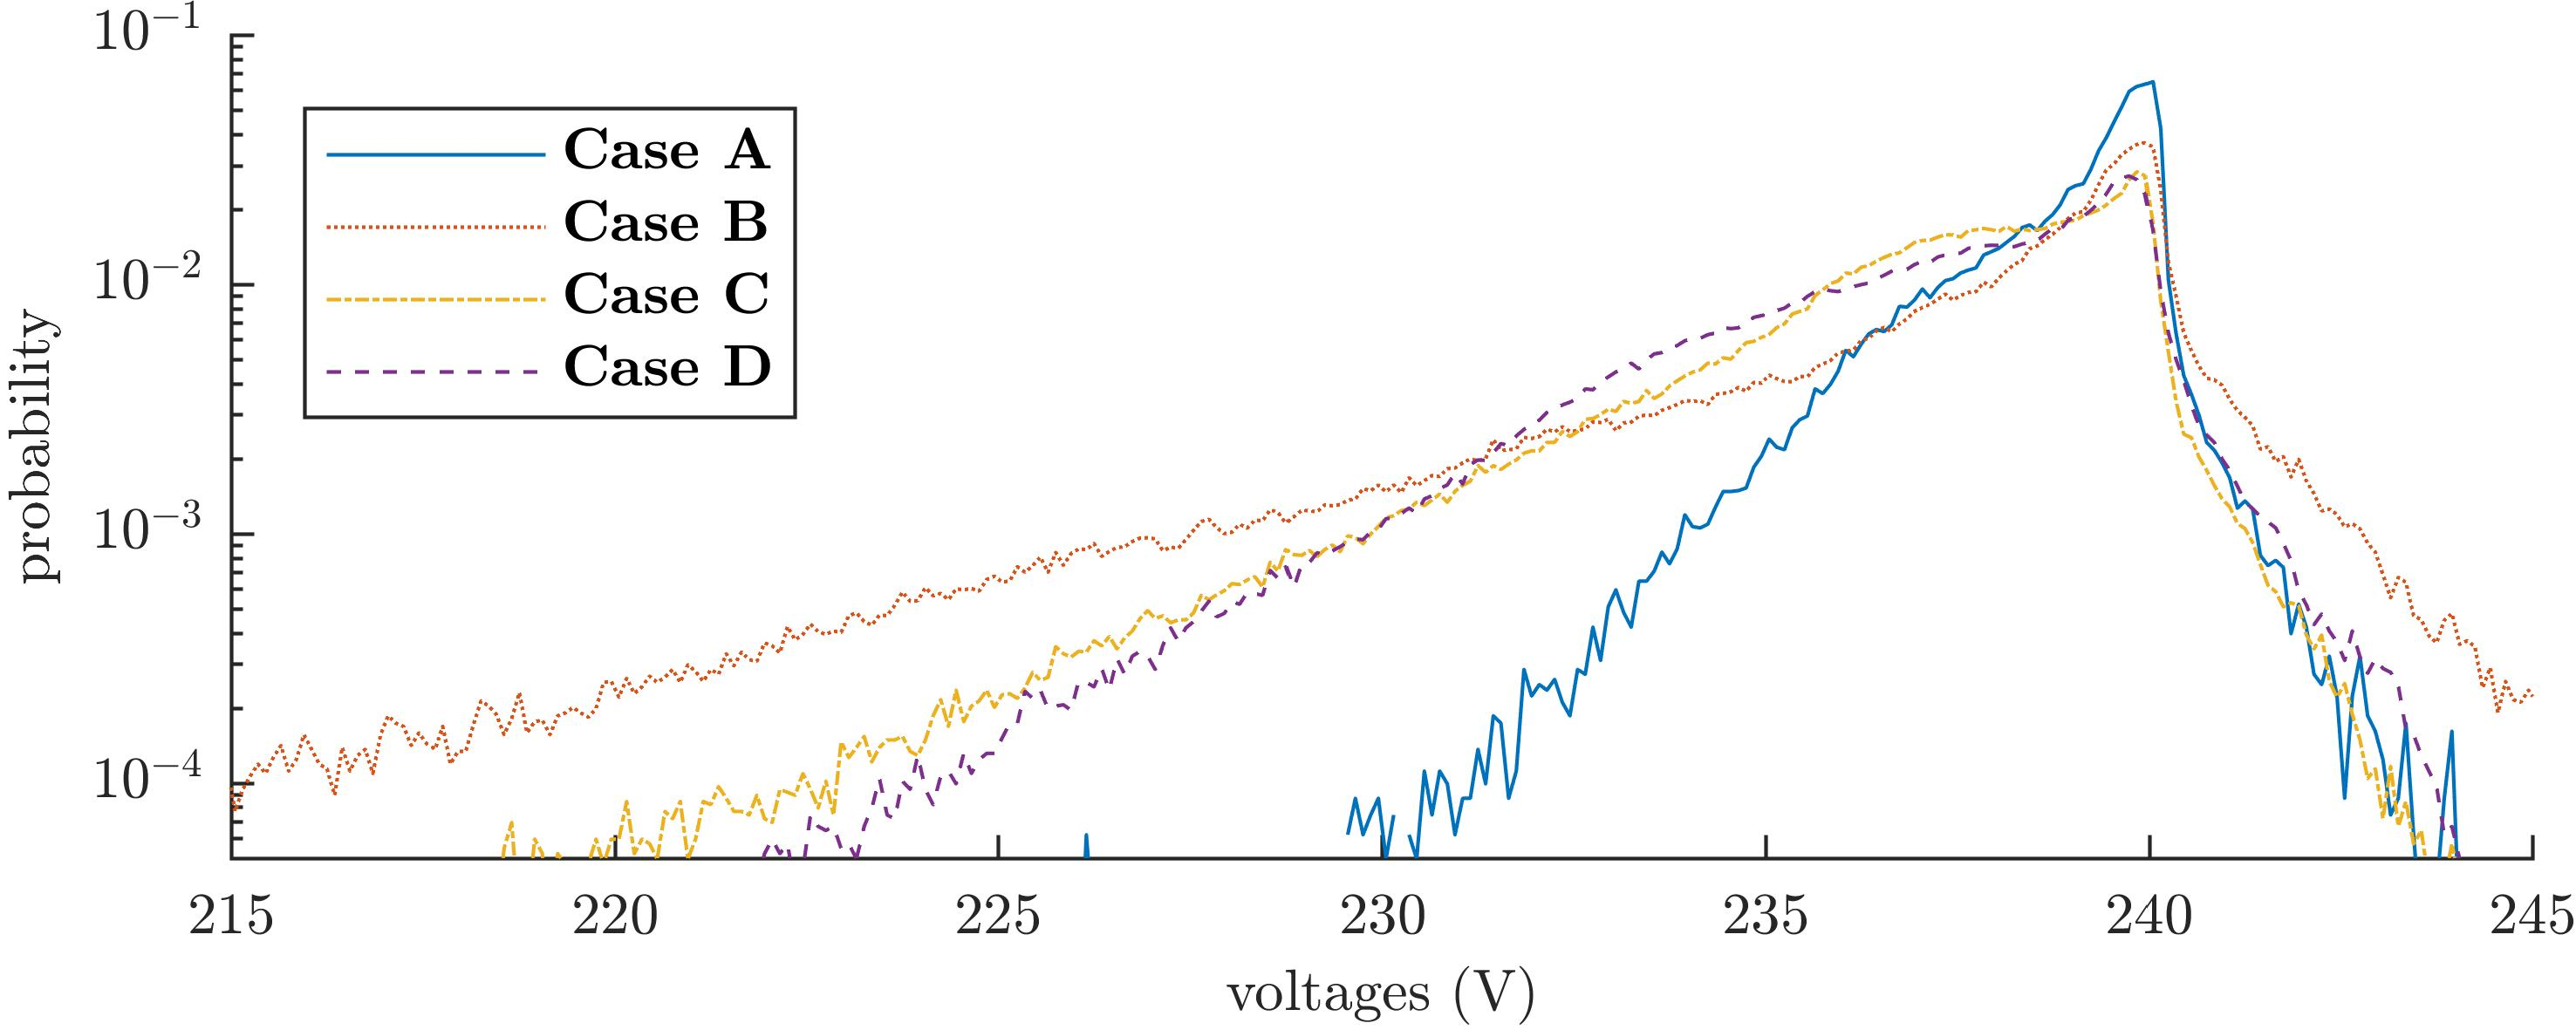
\includegraphics{_chapter4/fig/voltage-probabilities}
 \caption{Voltage level probability distribution for the entire feeder where\protect\linebreak $\zeta_\textbf{C}^{*}=-0.153$ and $\zeta_\textbf{D}^{*}=-0.135$.}
 \label{ch4:fig:voltage-probabilities}
\end{figure}


In this histogram, the voltage PD for all four cases were normalised and plotted against each other.
Here, the previously seen drop in voltages by introducing EVs is recorded as a shift in the voltage distribution towards the left.
The widened left hand tail of \ref{ch4:case-b} can be clearly observed in Figure~\ref{ch4:fig:voltage-probabilities}.
This voltage drop is then mitigated by the introduction of the storage solutions, since the voltage PD is shifted towards higher voltage bands, i.e. towards the right.
Since the difference between the BESS controlled by AIMD and AIMD+ is difficult to see, a comparison of their underlying performance metrics is necessary.
In Figure~\ref{ch4:fig:voltage-probabilities}, for the IEEE EU LV Test feeder, the AIMD+-controlled batteries outperform the AIMD devices since the resulting $\zeta_\textbf{C}^{*}$ is greater than $\zeta_\textbf{D}^{*}$.

\begin{figure}\centering
	\subfloat[]{
		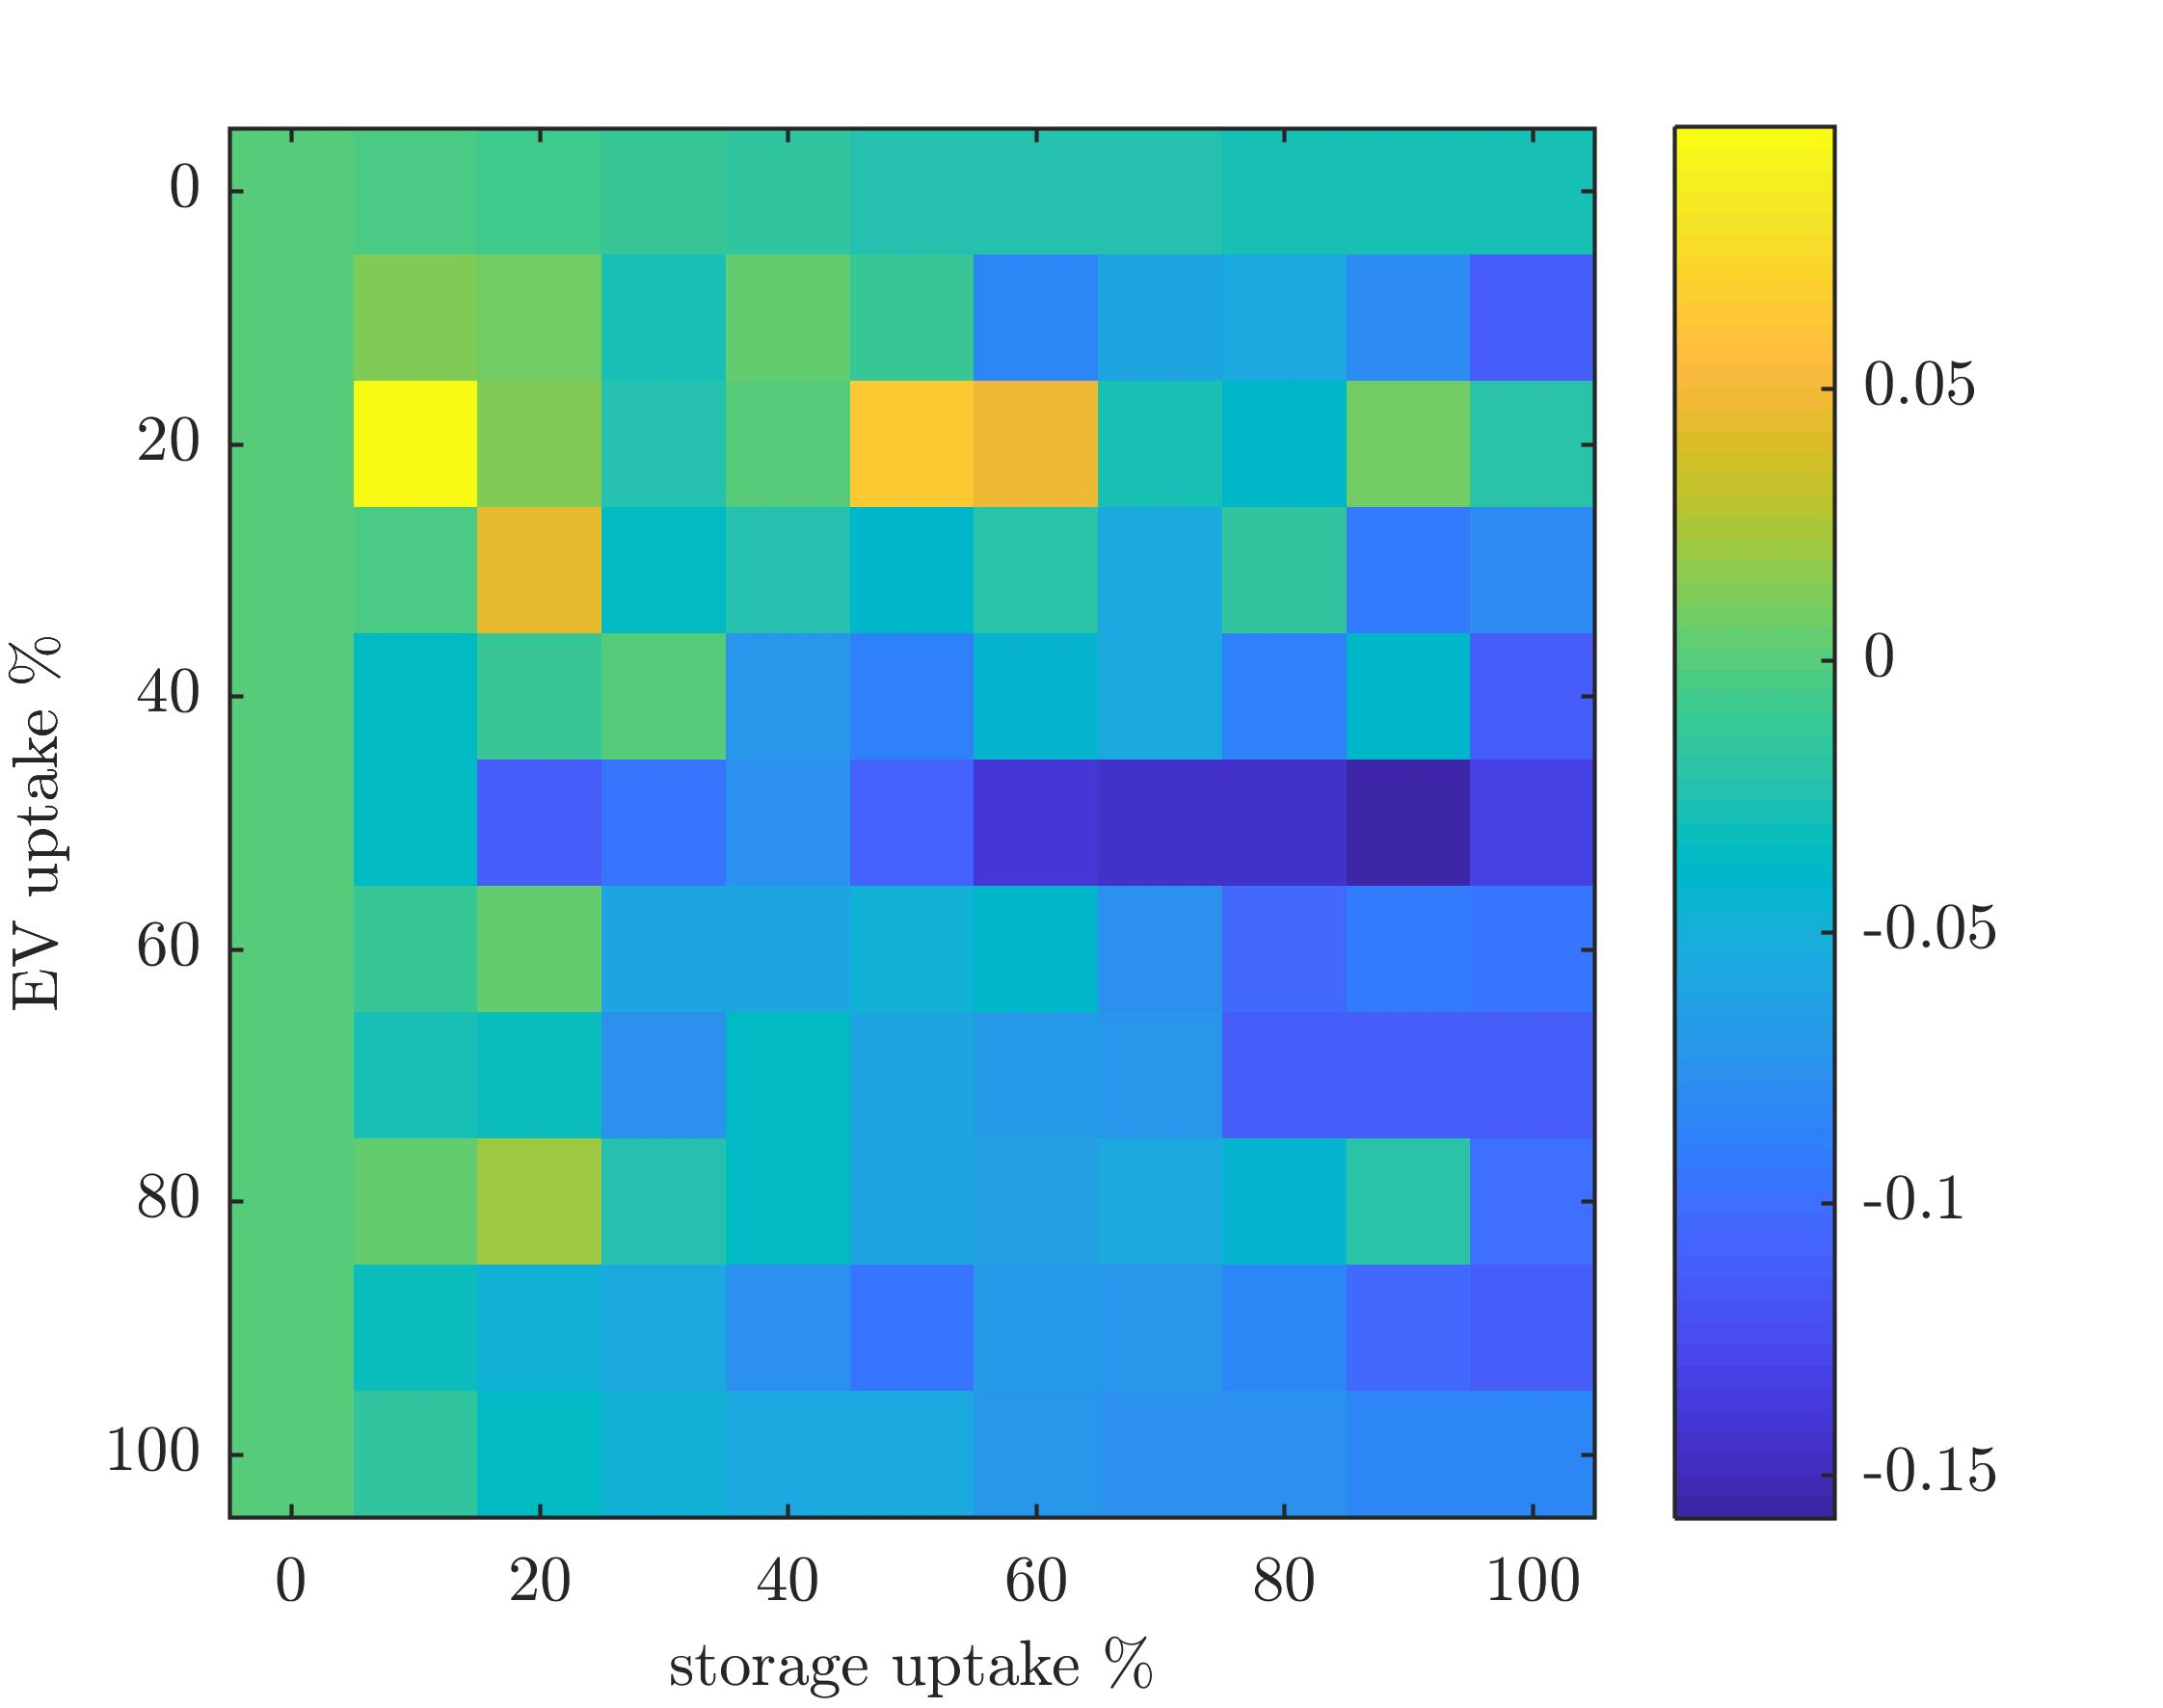
\includegraphics[width=0.5\textwidth]{_chapter4/fig/voltage-aimd}
		\label{ch4:subfig:voltage-aimd}
	}
	\subfloat[]{
		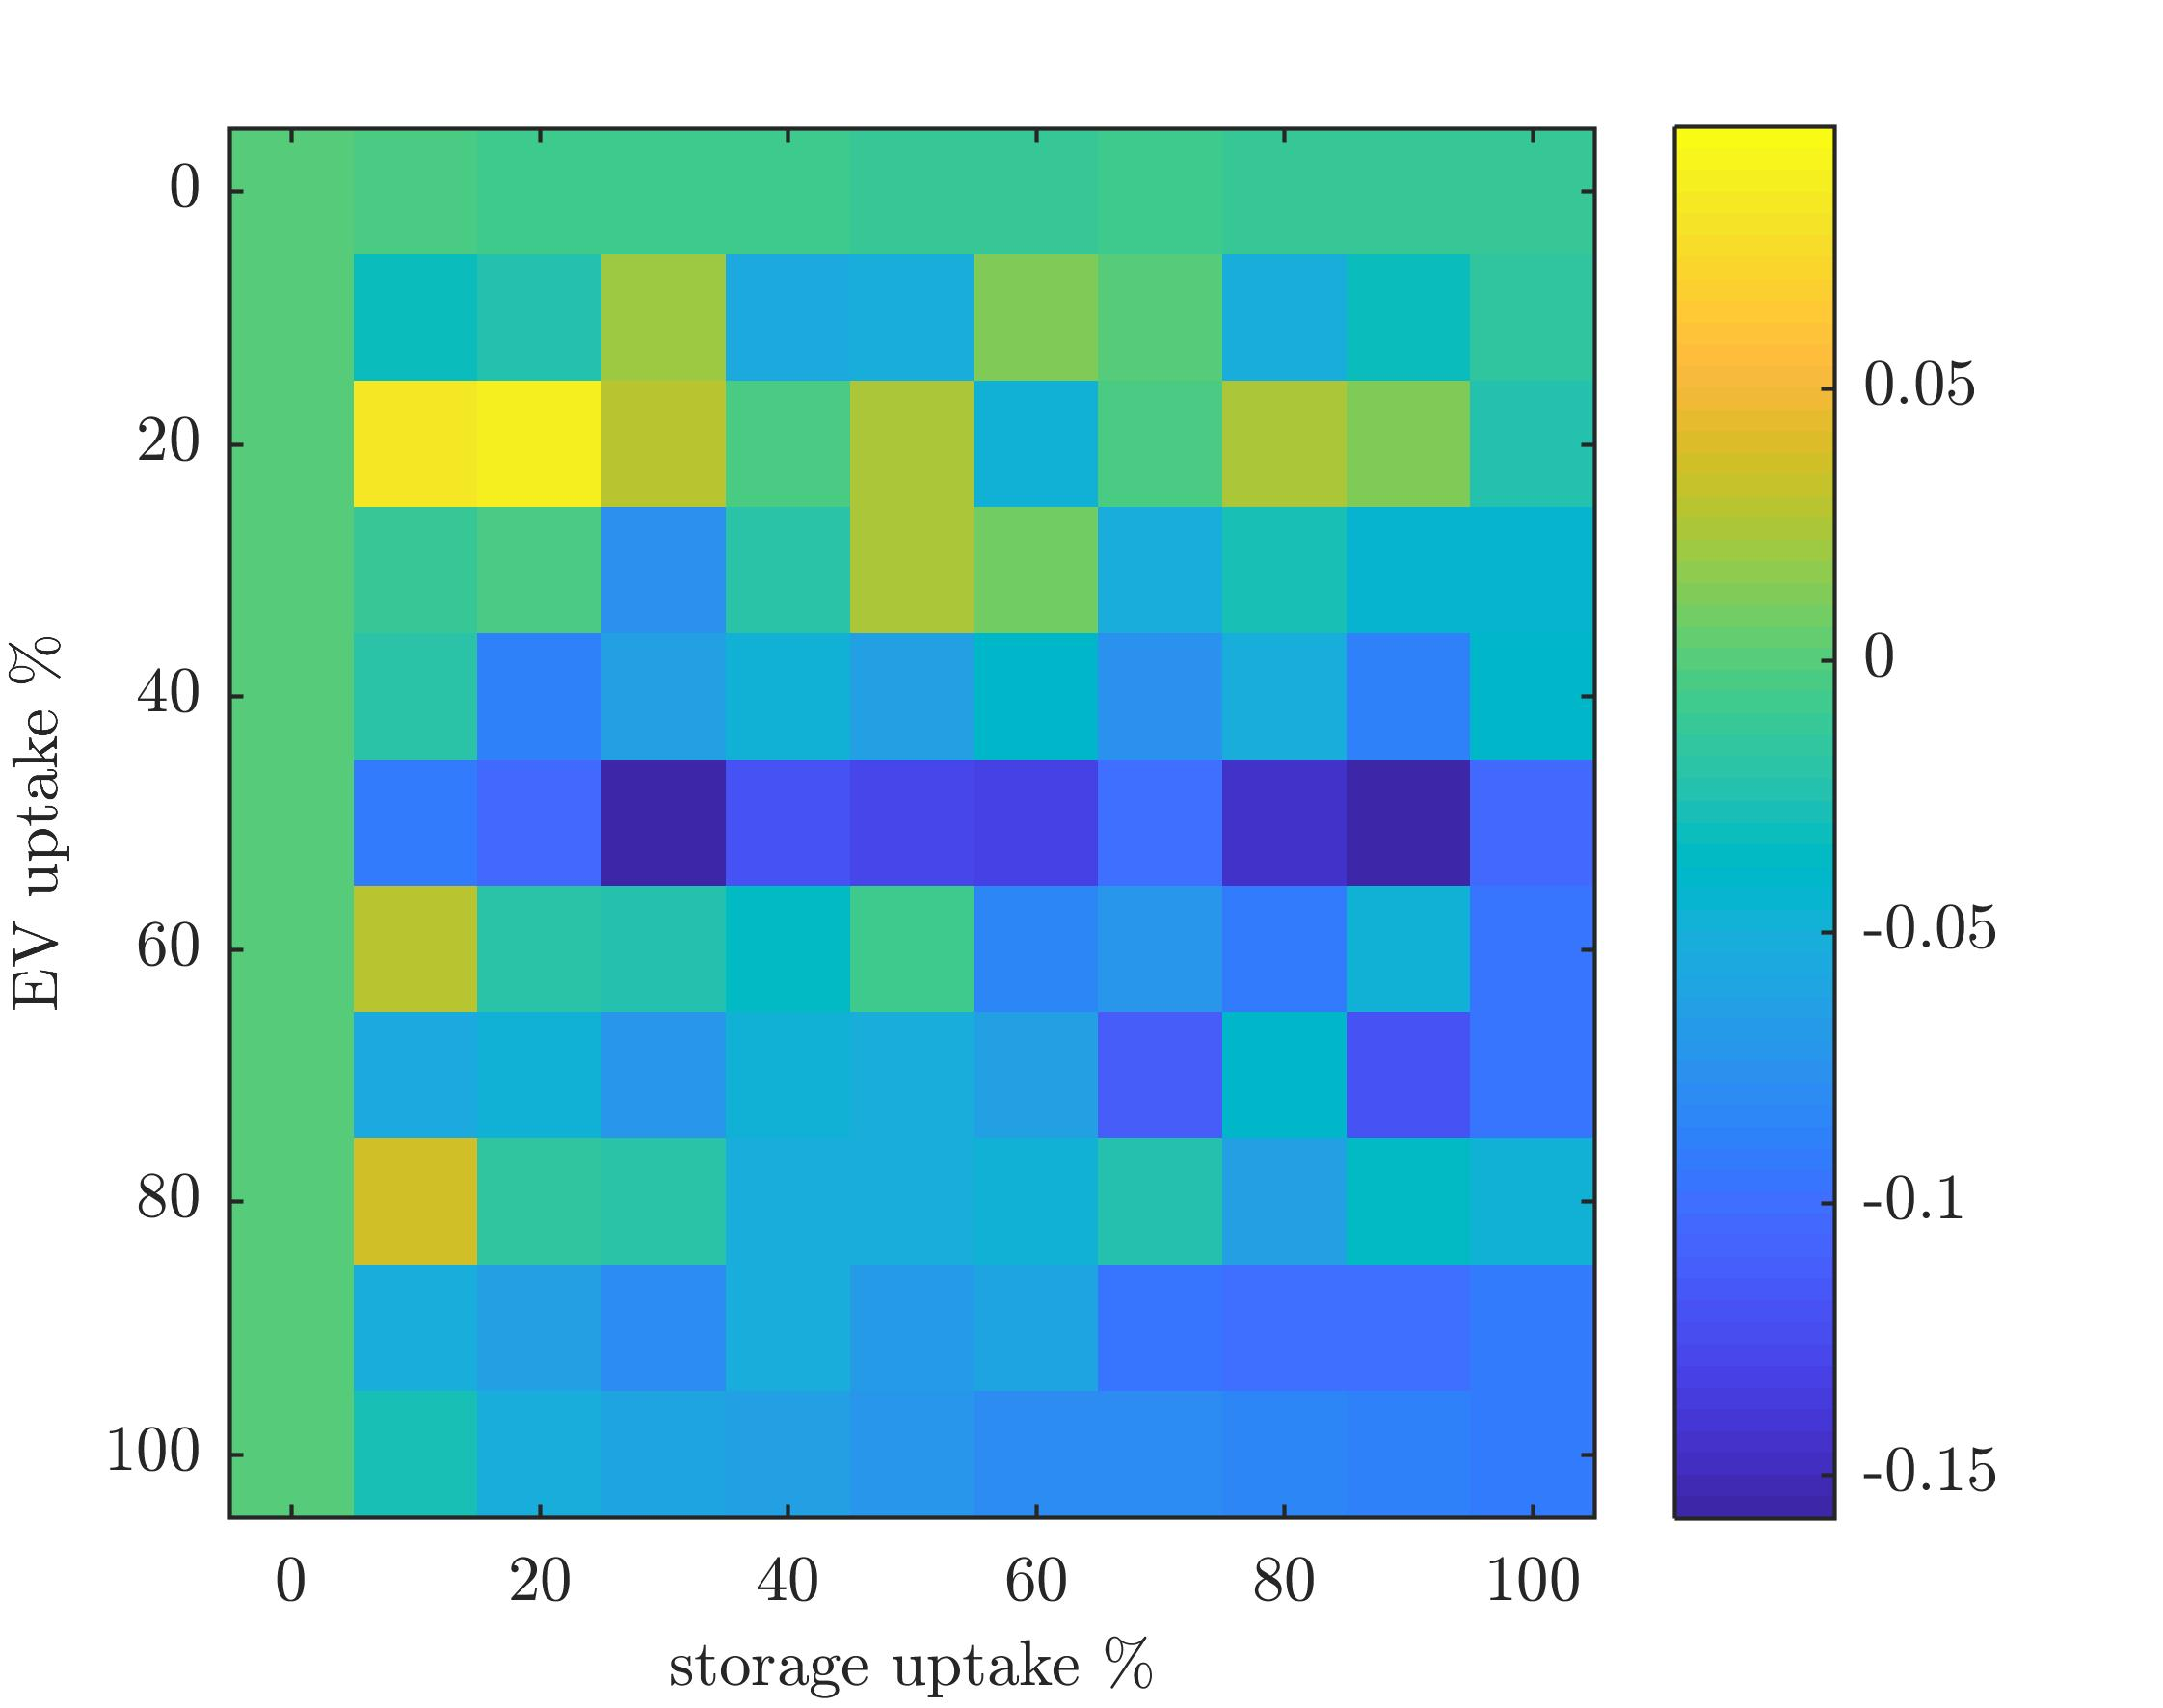
\includegraphics[width=0.5\textwidth]{_chapter4/fig/voltage-aimd-plus}
		\label{ch4:subfig:voltage-aimd-plus}
	}
	\caption{Comparison of voltage improvement indices for (a) $\zeta_\textbf{C}^{*}$ indices (AIMD); (b) $\zeta_\textbf{D}^{*}$ indices (AIMD+).}
	\label{ch4:fig:voltage-aimd}
\end{figure}


However, to gain a full understanding of the performance of the AIMD and AIMD+ algorithms, a full sweep of EV and BESS uptake combinations was simulated on all available power distribution networks.
The resulting parameters were averaged and plotted in Figure~\ref{ch4:fig:voltage-aimd}.

These figures show that the AIMD+ control algorithm reduces voltage deviation more effectively as the uptake in storage and EVs increases.
For low storage uptake, the AIMD algorithm does not perform as strongly since more $\zeta_\textbf{C}^{*}$ values are positive and larger than their corresponding $\zeta_\textbf{D}^{*}$ value.
This becomes more apparent when averaging all $\zeta_\textbf{C}^{*}$ and $\zeta_\textbf{D}^{*}$ values for their common storage uptake and across all EV uptakes.
The resulting averaged metrics are plotted in Figure~\ref{ch4:fig:voltage-aimd-compare}.

\begin{figure}\centering
	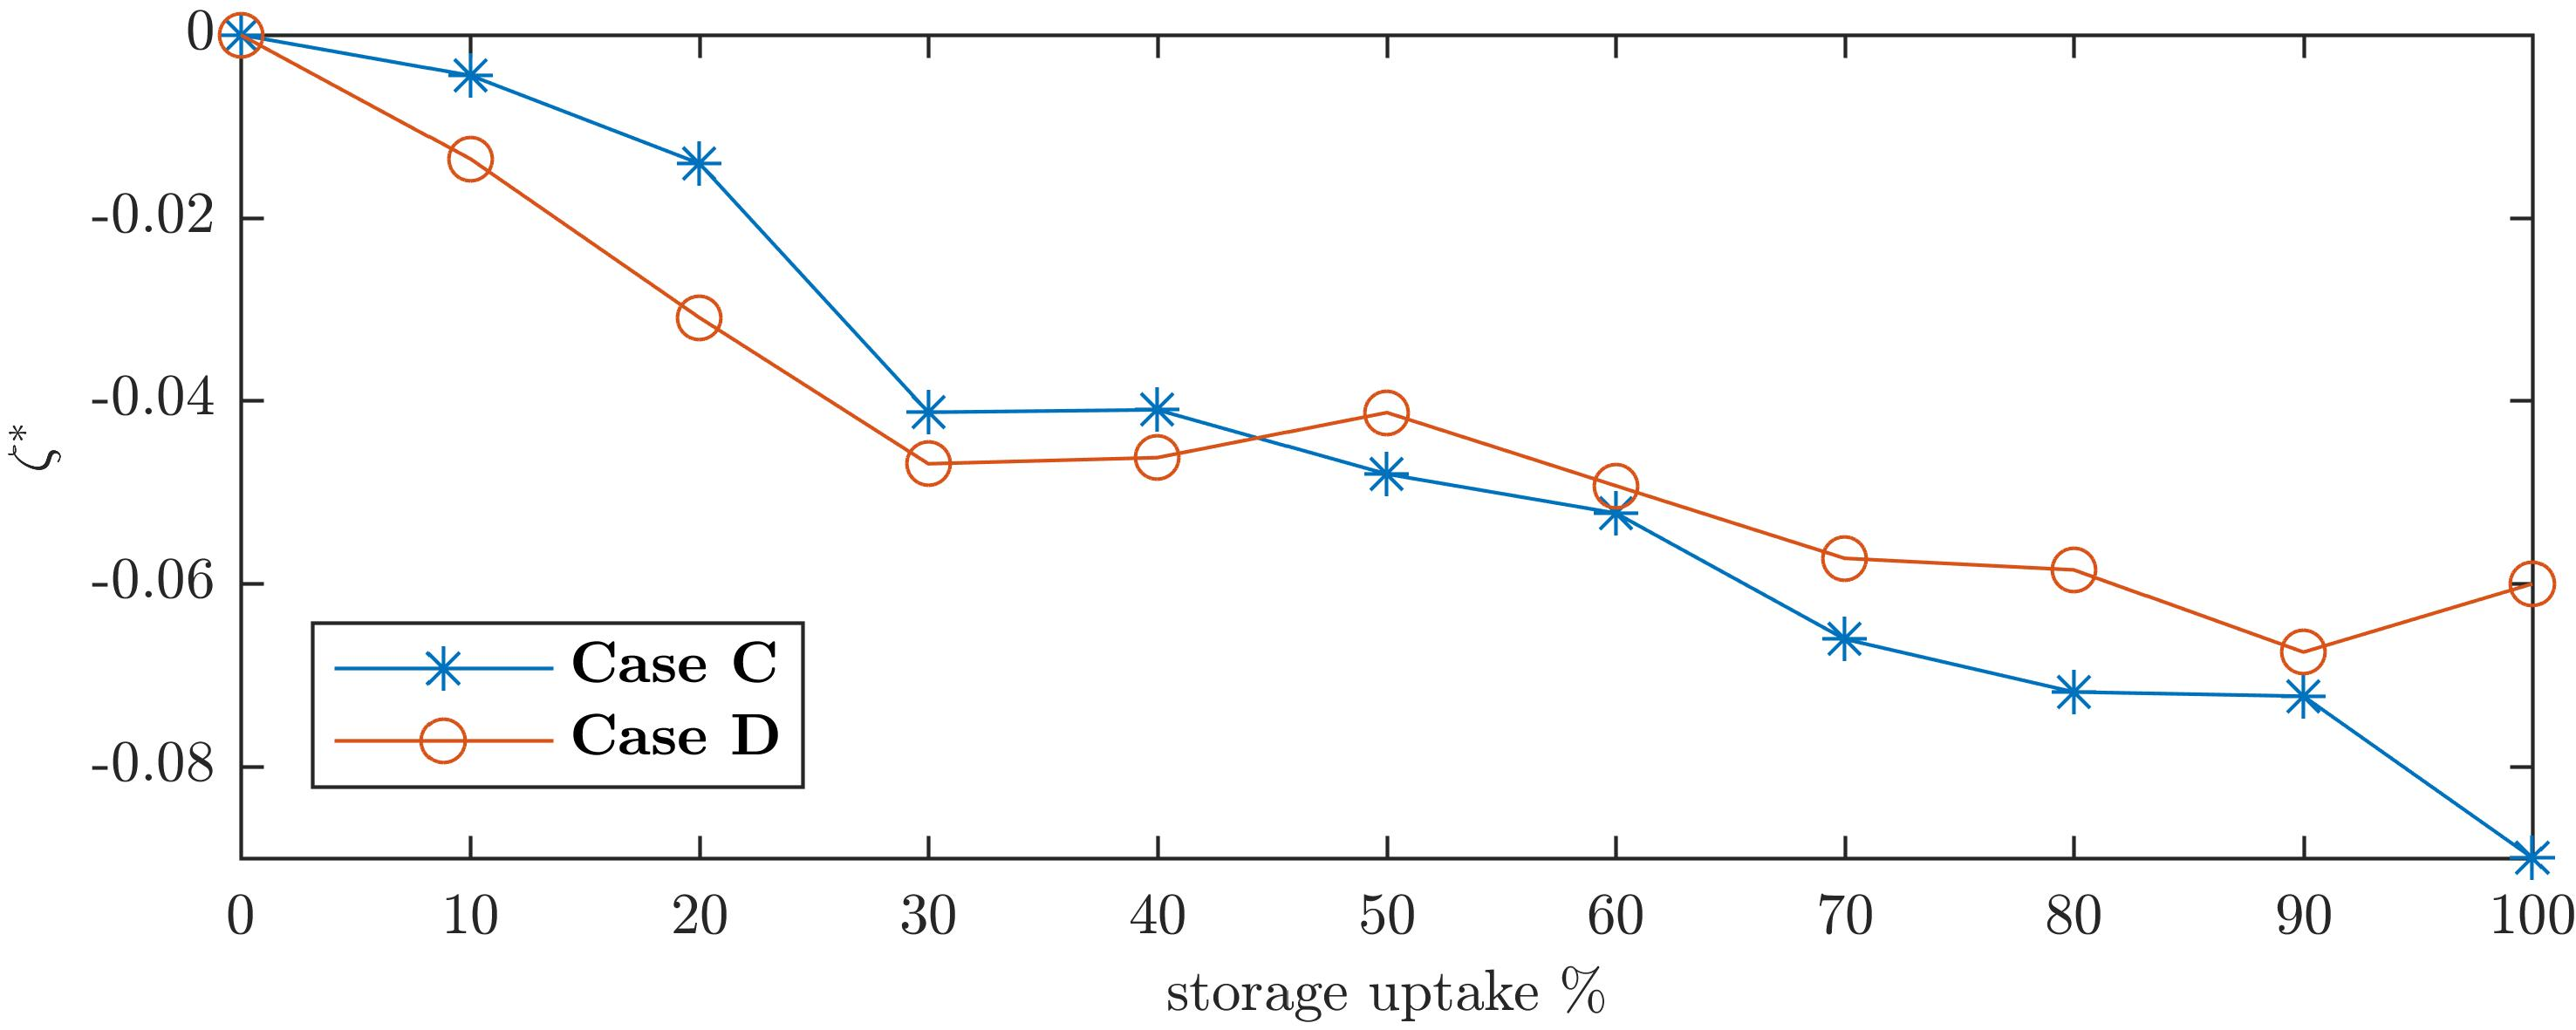
\includegraphics{_chapter4/fig/voltage-aimd-compare}
	\caption{Average $\zeta_\textbf{C}^{*}$ and $\zeta_\textbf{D}^{*}$ values recorded against the corresponding storage uptake.}
	\label{ch4:fig:voltage-aimd-compare}
\end{figure}


In this last figure, Figure~\ref{ch4:fig:voltage-aimd-compare}, it can be seen how the sole impact of BESS uptake reflects in a continuing improvement of voltage levels.
In fact, both compared algorithms improved the bus voltage, which coincides with the findings in the case studies.
On average, this is the case for all BESS uptakes, as $\zeta_\textbf{C}^{*} \approx \zeta_\textbf{D}^{*}$.
Nonetheless, it should be noted that the AIMD+ algorithm had reduced the frequency of severe voltage deviations in comparison to the AIMD algorithm and is more effective during scenarios with lower BESS uptake.

\subsection{Line Overload Analysis}

\begin{figure}\centering
	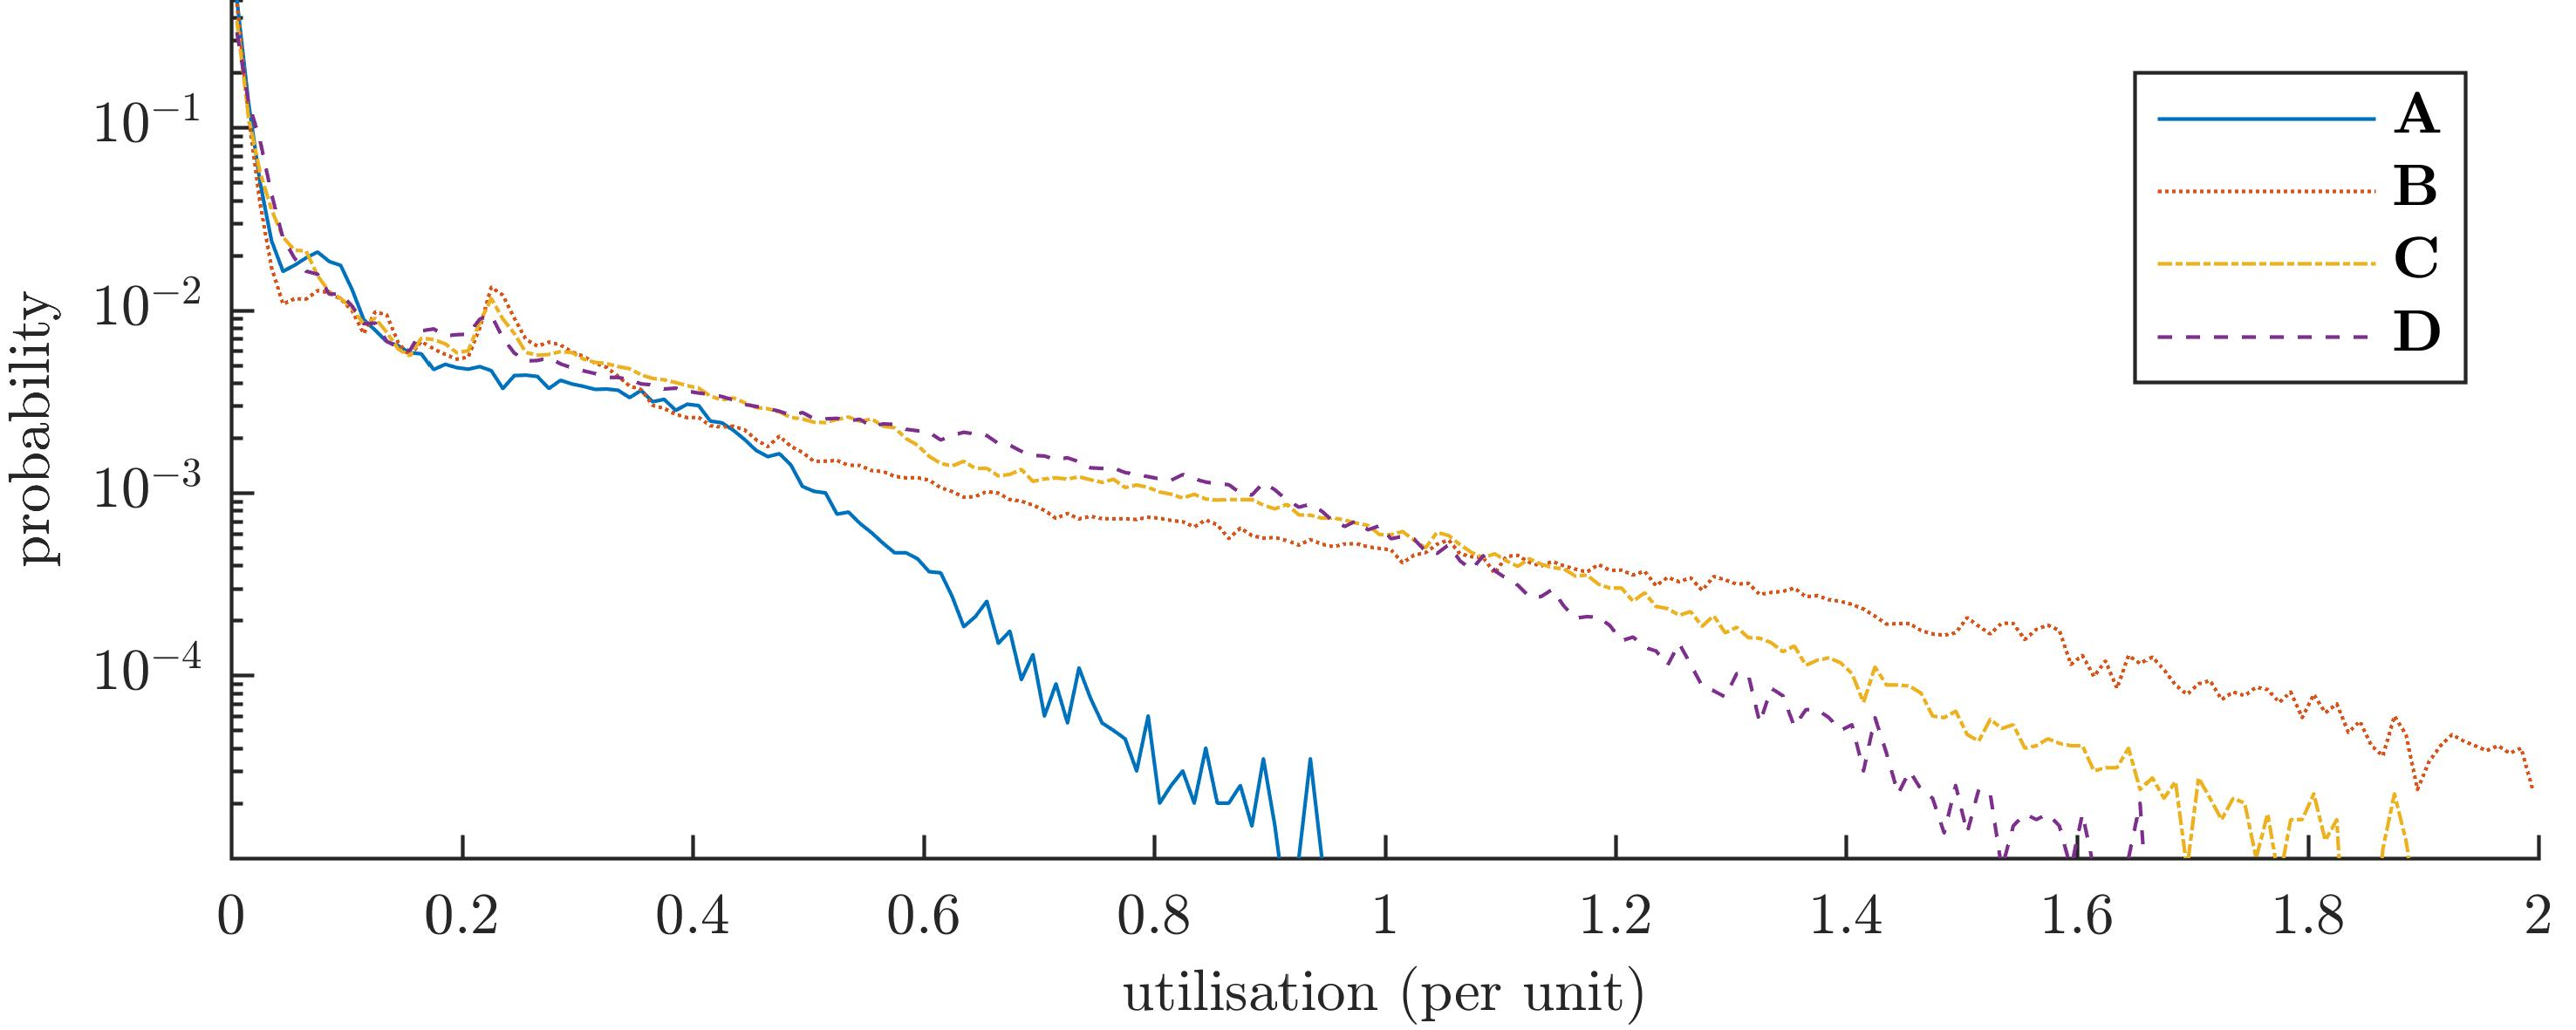
\includegraphics{_chapter4/fig/utilisation-probability}
	\caption{Line utilisation probability distribution of all lines in the simulated feeder where $\zeta_\textbf{C}^{**}=-0.360$ and $\zeta_\textbf{D}^{**}=-0.518$.}
	\label{ch4:fig:utilisation-probability}
\end{figure}


Similar to the voltage PD analysis, a PD of the line utilisation was generated and plotted in Figure~\ref{ch4:fig:utilisation-probability}.
This figure shows a normalised PD plot of the per unit current in all lines, for each of the four scenarios (here, 1 p.u. represents a 100\% line usage, i.e., a line current of the same value as the line's nominal current rating).
Whilst the case without any charging EVs, i.e. \ref{ch4:case-a}, shows no overloading, \ref{ch4:case-b} has significantly widened the probability spectrum.
AIMD and AIMD+ controlled BESS can mitigate the effect of this EV introduction, and the difference in performance becomes more apparent than it did for the voltage PD analysis.
In Figure~\ref{ch4:fig:utilisation-probability} the PDs for \ref{ch4:case-c} and \ref{ch4:case-d} intersect at 1 p.u. load, yet for the AIMD+ scenario, overloads are less likely than for the AIMD controlled scenario.
However, in this figure it can also be observed that the used test network is of insufficient capacity to cater for the chosen EV uptake, since the probability of line over-utilisation is still above zero.

Nonetheless, the AIMD+ controlled storage devices yielded a noticeable reduction in line overloads, despite being a voltage driven control method.
This improvement is apparent through the compressed width of the probability distribution and the negative $\zeta_\textbf{D}^{**}$ value.
In contrast, the AIMD controlled storage devices do not fully utilise the line capacity as effectively, which leads to a positive value of $\zeta_\textbf{C}^{**}$.
To evaluate the line utilisation improvement across all simulations, the full range of EV and storage uptake was evaluated. The resulting plots are shown in Figure~\ref{ch4:fig:utilisation-aimd}.

\begin{figure}\centering
\subfloat[]{
	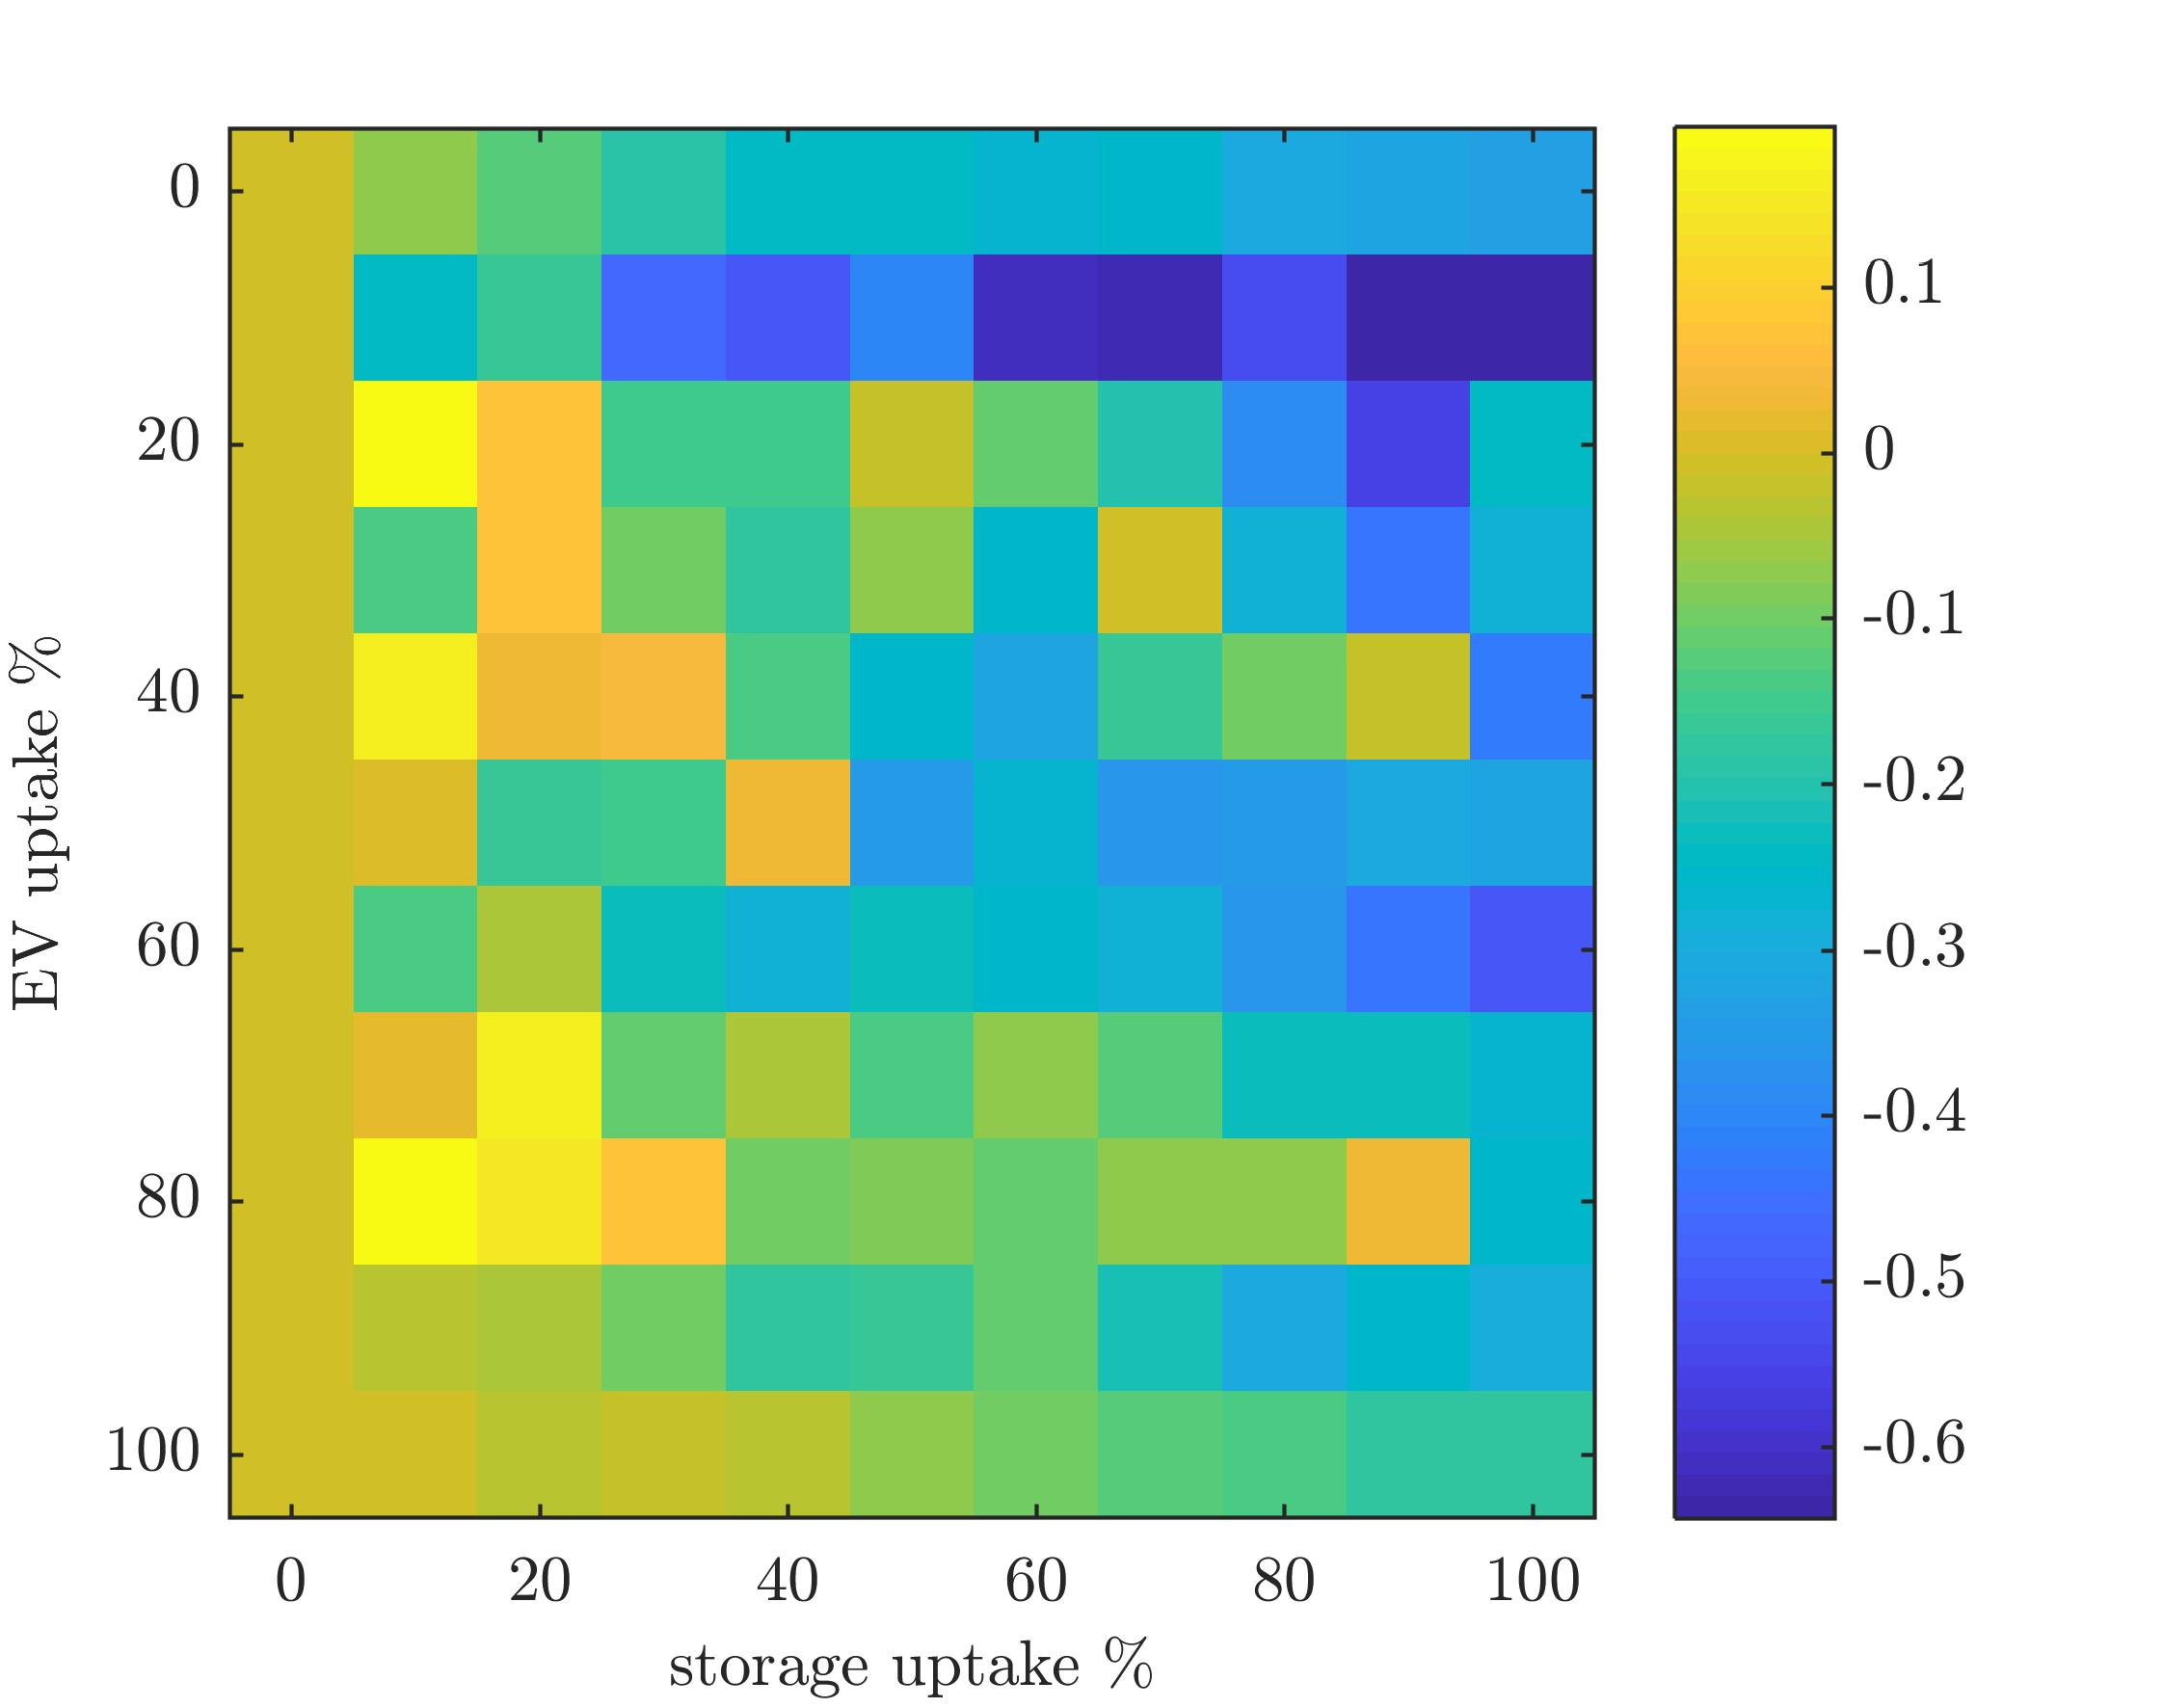
\includegraphics[width=0.5\textwidth]{_chapter4/fig/utilisation-aimd}
	\label{ch4:subfig:utilisation-aimd}
}
\subfloat[]{
	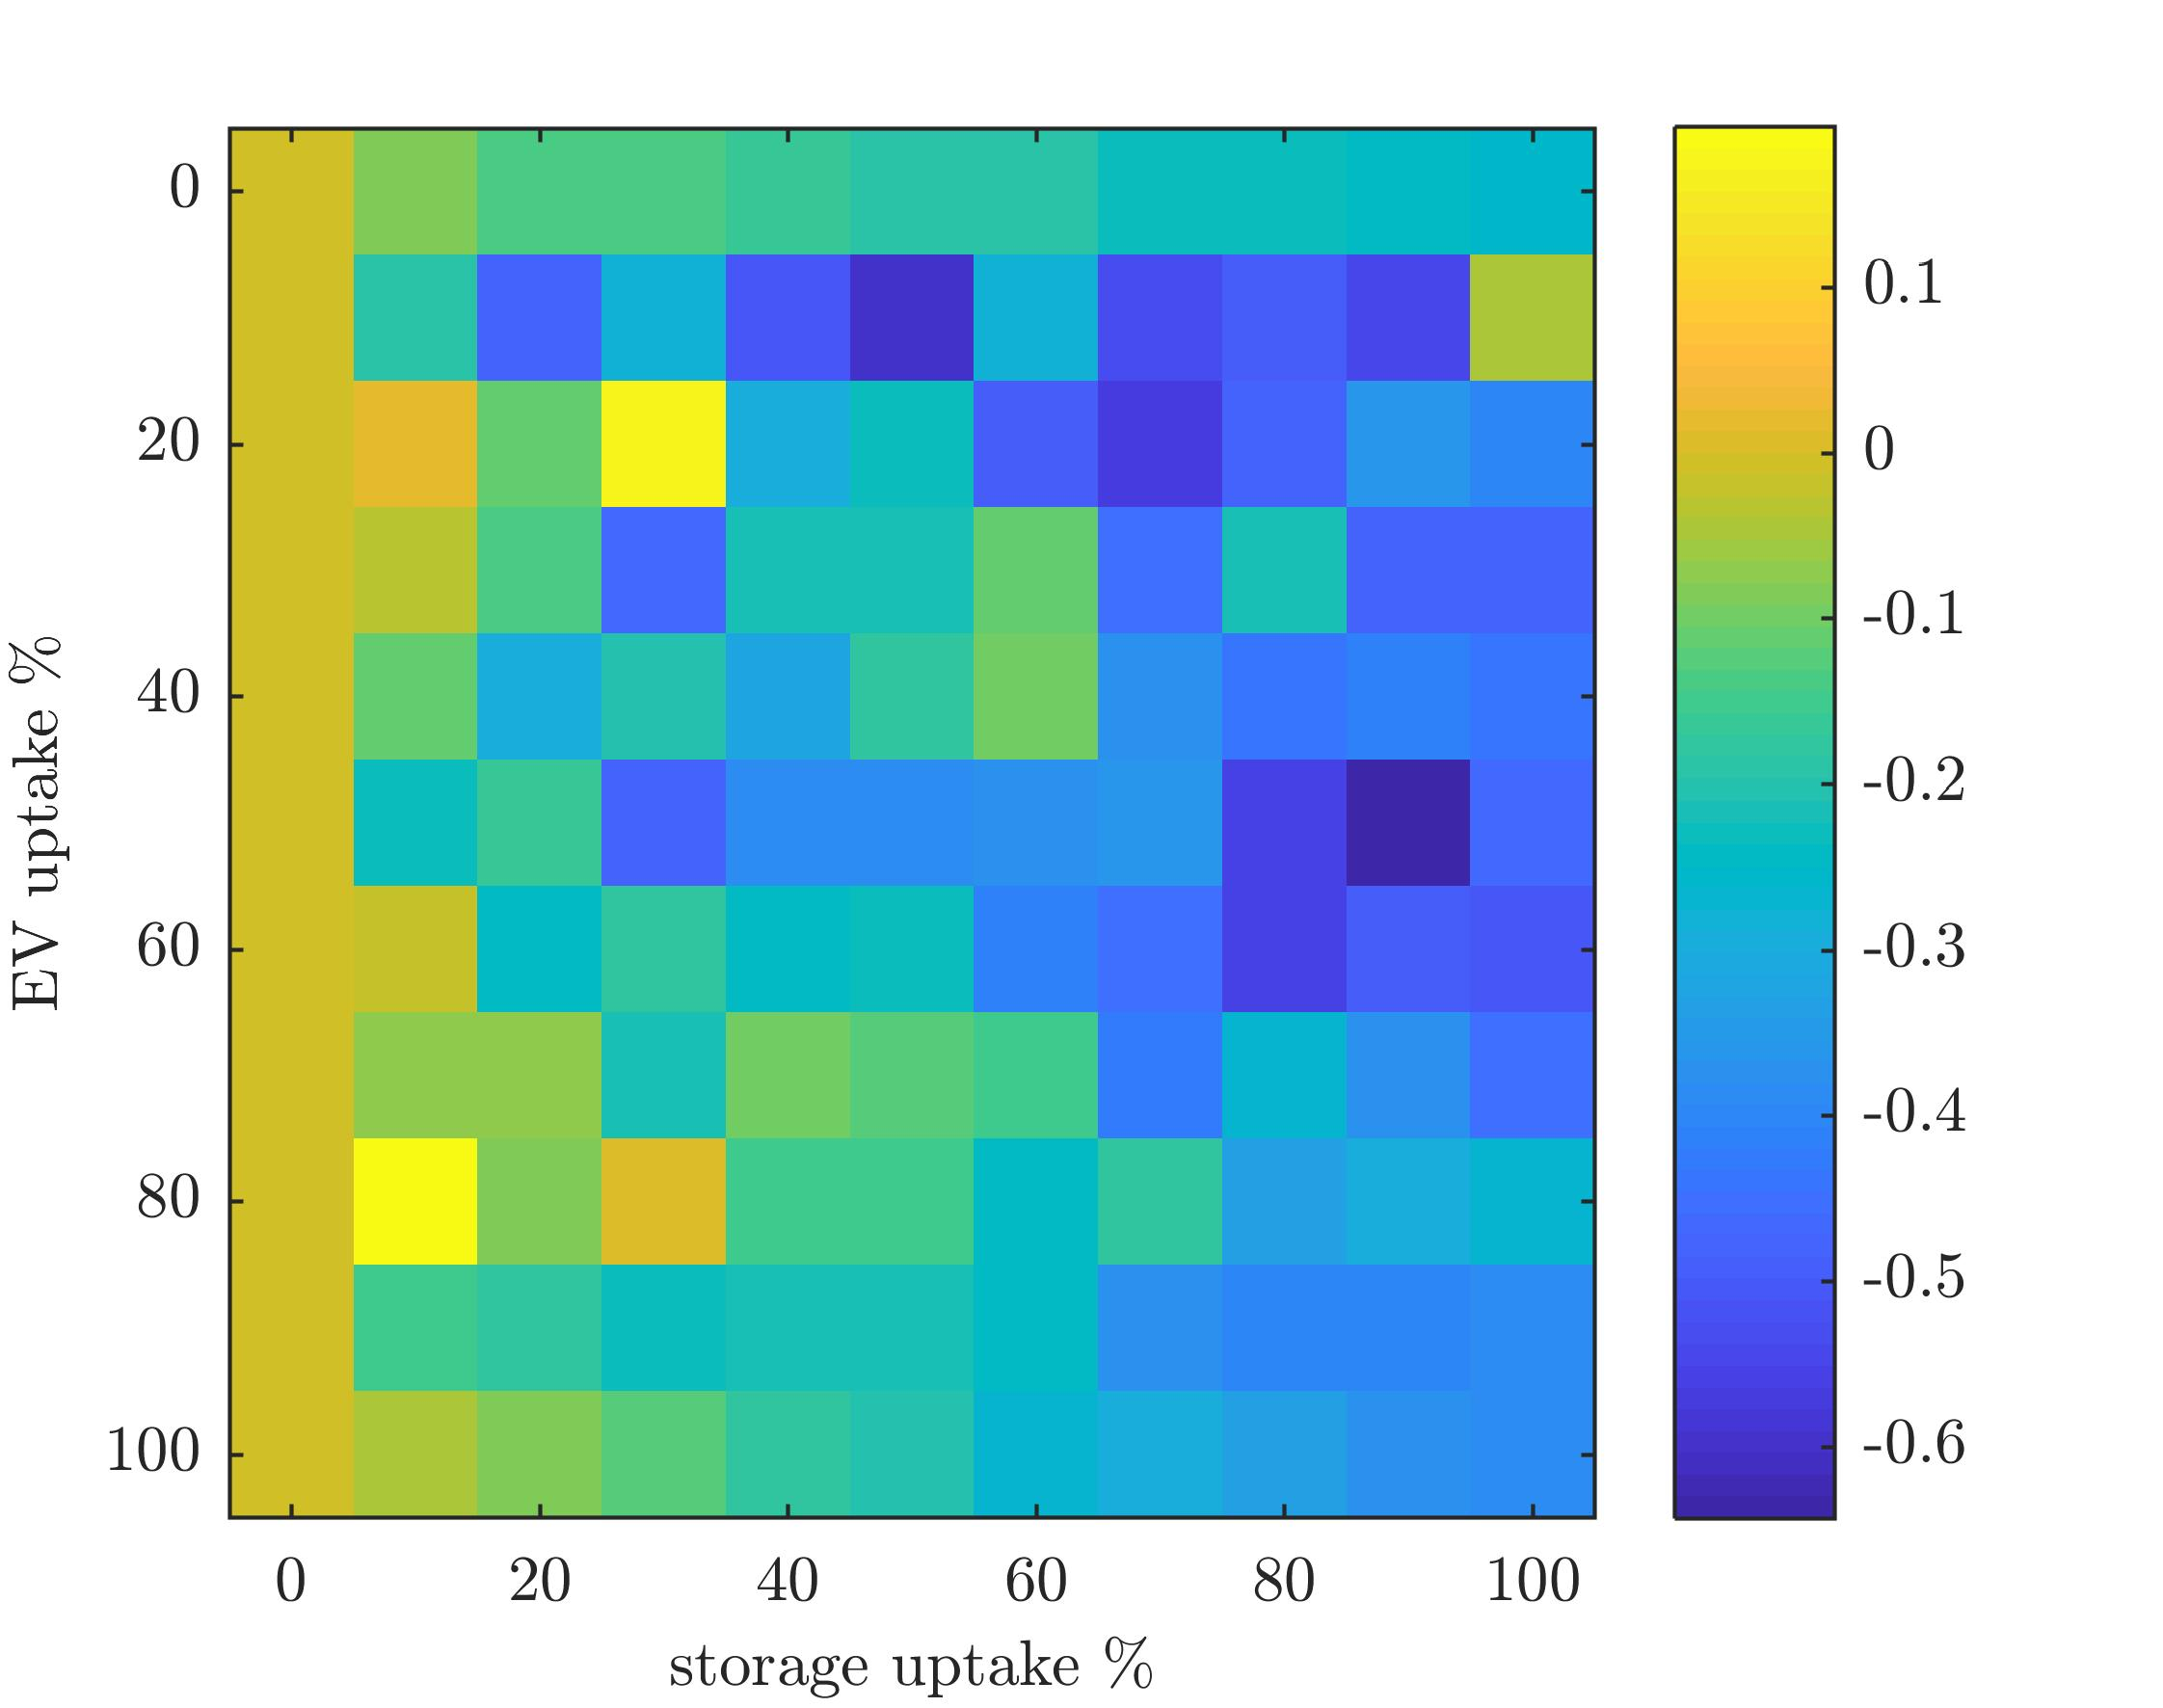
\includegraphics[width=0.5\textwidth]{_chapter4/fig/utilisation-aimd-plus}
	\label{ch4:subfig:utilisation-aimd-plus}
}
\caption{Comparison of line utilisation improvement indices for (a) $\zeta_\textbf{C}^{*}$ indices (AIMD); (b) $\zeta_\textbf{D}^{*}$ indices (AIMD+).}
\label{ch4:fig:utilisation-aimd}
\end{figure}


In these figures, it can be seen how the performance metrics change as EV uptake and storage uptake increase.
For the AIMD-controlled BESS, the resulting $\zeta_\textbf{C}^{**}$ values are distributed around zero, whereas the AIMD+ algorithm achieved negative values of $\zeta_\textbf{D}^{**}$ for nearly 90\% of the performed simulations.
These negative values confirm the better usage of available line capacity. This becomes particularly apparent for scenarios where very low EV uptake is combined with larger BESS uptake.
Here, AIMD-controlled storage devices commence their initial charge simultaneously.
As they are located closer to the substation, they do not measure a sufficient bus voltage offset to regulate down their charging power.
This behaviour causes a number of line overloads at the very beginning of the simulated days.
The AIMD+ algorithm on the other hand, with its adjusted thresholds, is more responsive to non-optimal network operation and, therefore, increases the charging rate gradually.

\begin{figure}\centering
	 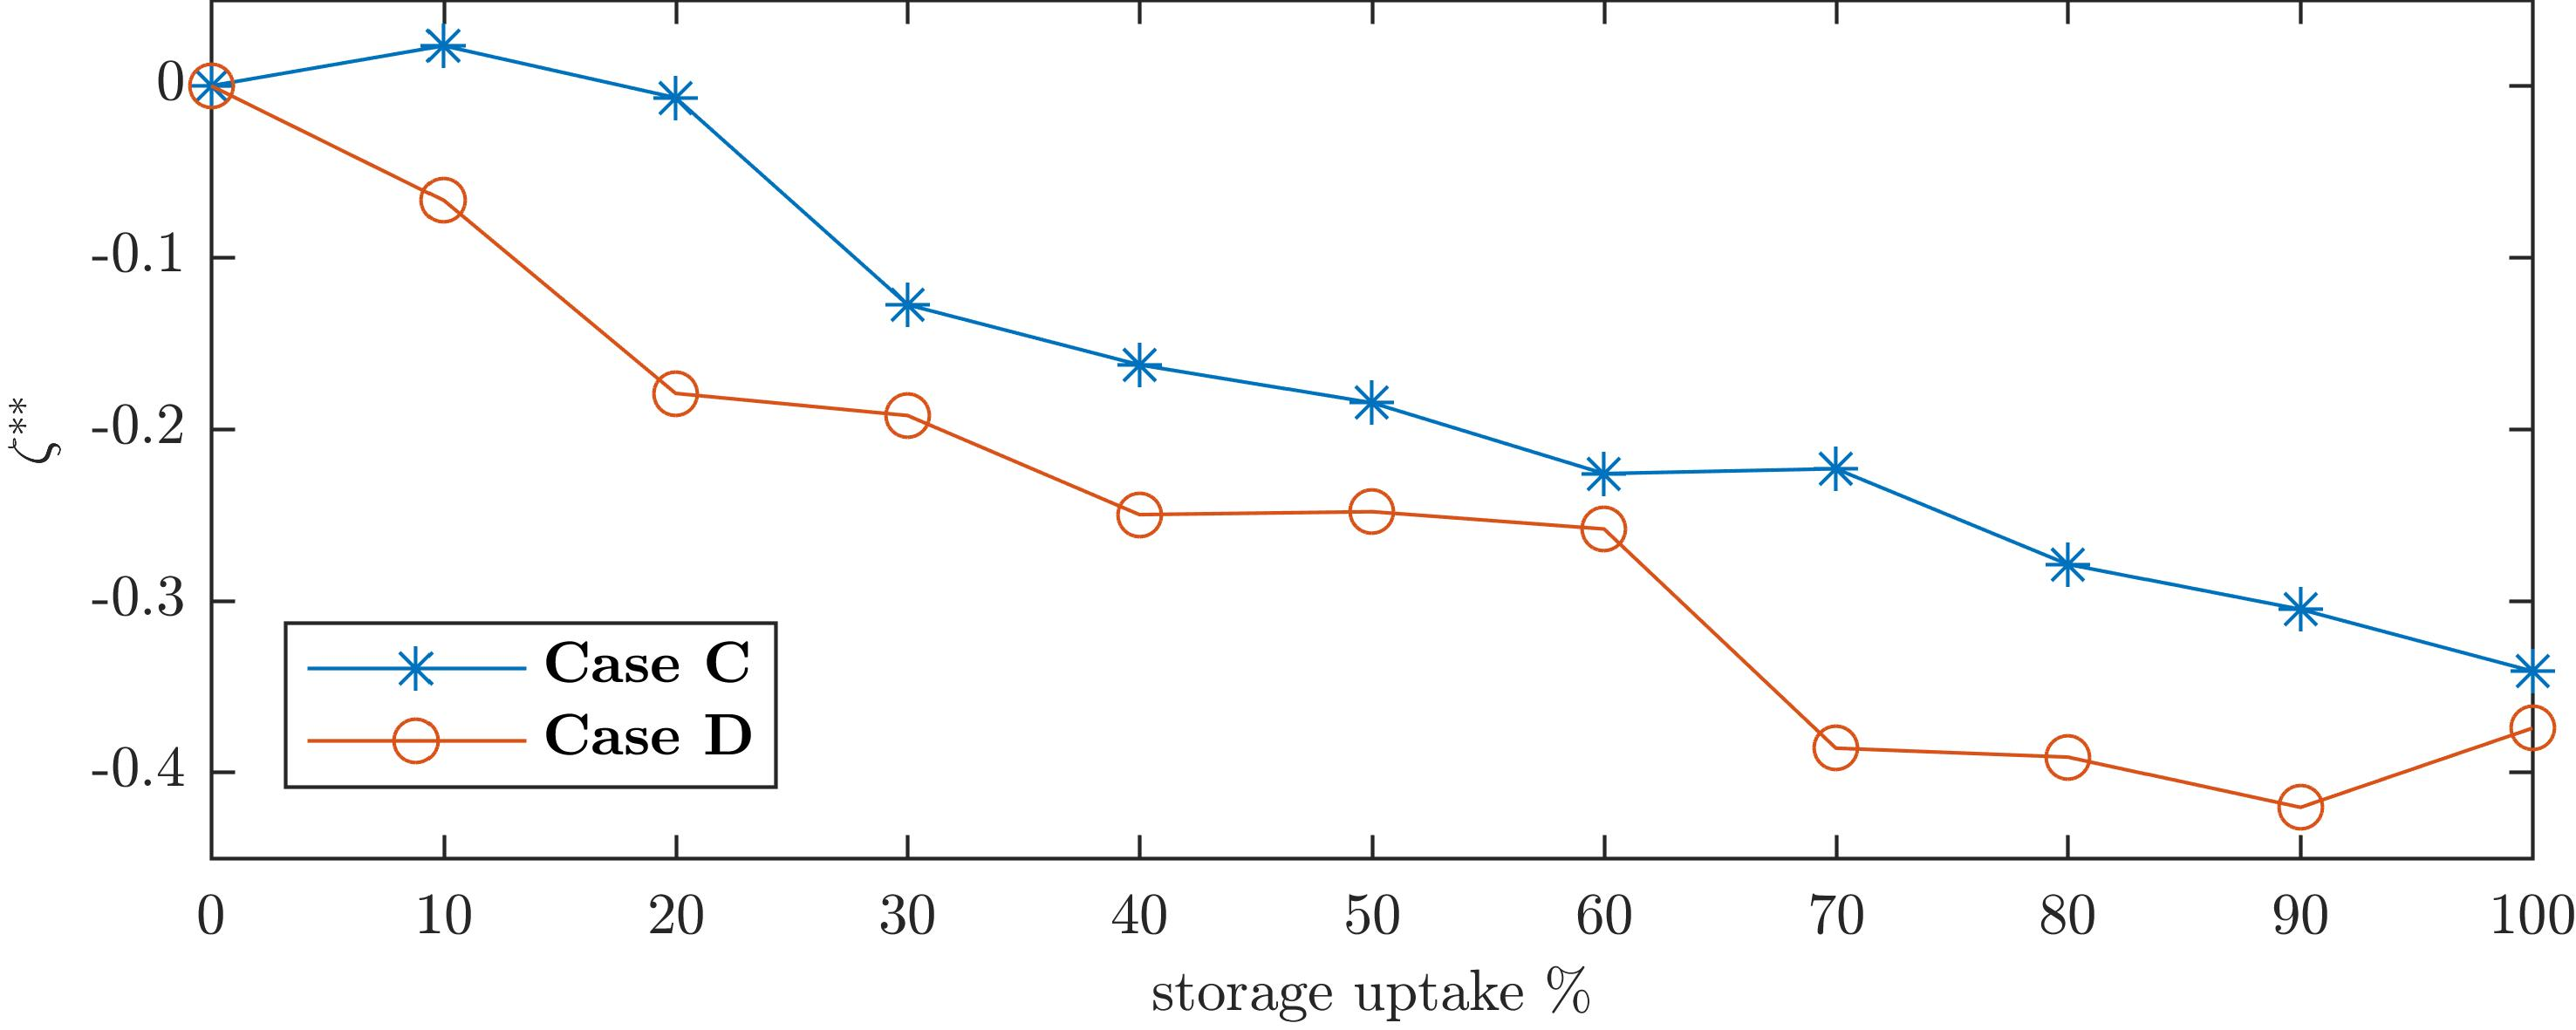
\includegraphics{_chapter4/fig/utilisation-aimd-compare}
	 \caption{Average $\zeta_\textbf{C}^{**}$ and $\zeta_\textbf{D}^{**}$ values recorded against the corresponding storage uptake.}
	 \label{ch4:fig:utilisation-aimd-compare}
\end{figure}


This gradual adjustment is based on the fact that the bus voltages in the AIMD+ algorithm are closer to their nominal voltages (i.e., bus voltages found by simulating the feeder with its equally-distributed nominal load) than they are in the conventional AIMD case.
A greater voltage disparity, which is the case in AIMD, causes a prolonged additive adjustment to the battery's power.
This prolonged adjustment is particularly apparent for batteries situated at the bottom of the feeder, as their voltage measurements deviate the furthest from the substation voltage level.
AIMD+ on the other hand prevents this behaviour by setting the voltage threshold based on the network's nominal voltage drop, which is dependent on the distance between the BESS and its feeding substation.
As a result, the set-point voltage thresholds at the bottom of the feeder are lower than those closer to the substation.
Hence, the additive power adjustment becomes equal for all BESS along the feeder.
Therefore, by applying these individualised control thresholds, the sensitivity of the algorithm is corrected, whilst successfully mitigating the severity of line overloads.

Averaging the $\zeta_\textbf{C}^{**}$ and $\zeta_\textbf{D}^{**}$ values over all EV uptakes gives a clearer indication of performance, as this is now the only variable in the performance analysis.
The result is plotted in Figure~\ref{ch4:fig:utilisation-aimd-compare}.
Here, the hypothesis that AIMD-controlled energy storage devices do not improve line utilisation is confirmed.
In contrast, the AIMD+-controlled devices succeed at effectively reducing line overloads.
This is also demonstrated by the values of $\zeta_\textbf{C}^{**}$, which remain positive yet close to zero, whereas $\zeta_\textbf{D}^{**}$ decreases with increasing uptake of battery storage devices, as shown in Figure~\ref{ch4:fig:utilisation-aimd-compare}.

Whilst the deployment of energy storage has often been seen as a possible solution to defer network reinforcements, the presented results show that this is not always the case.
In fact, due to technical limitations, choosing an appropriate control algorithm enables the BESS to perform optimally.
This becomes particularly apparent when, e.g. energy storage devices need to recharge their injected energy for times of peak demand.
For the AIMD case, this recharging was not controlled in accordance to the underlying network properties, which led to higher line currents.
The proposed AIMD+ algorithm was not as susceptible to this kind of behaviour, as it has been designed to take battery location into account.
This immunity and well-controlled power flow caused little to no additional strain on the network's equipment, allowing the deployed storage devices to also provide voltage support.

\subsection{Battery Utilisation Analysis}

In this part of the analysis, the batteries' equality of use was evaluated by comparing the battery cycling for each AIMD implementation.
As already mentioned, a single battery cycle is defined as a full discharge and recharge.
In Figure~\ref{ch4:fig:storage-aimd}, the battery power profiles are plotted along the horizontal axis and they are order by increasing distance to the substation:

\begin{figure}\centering
	\subfloat[]{
		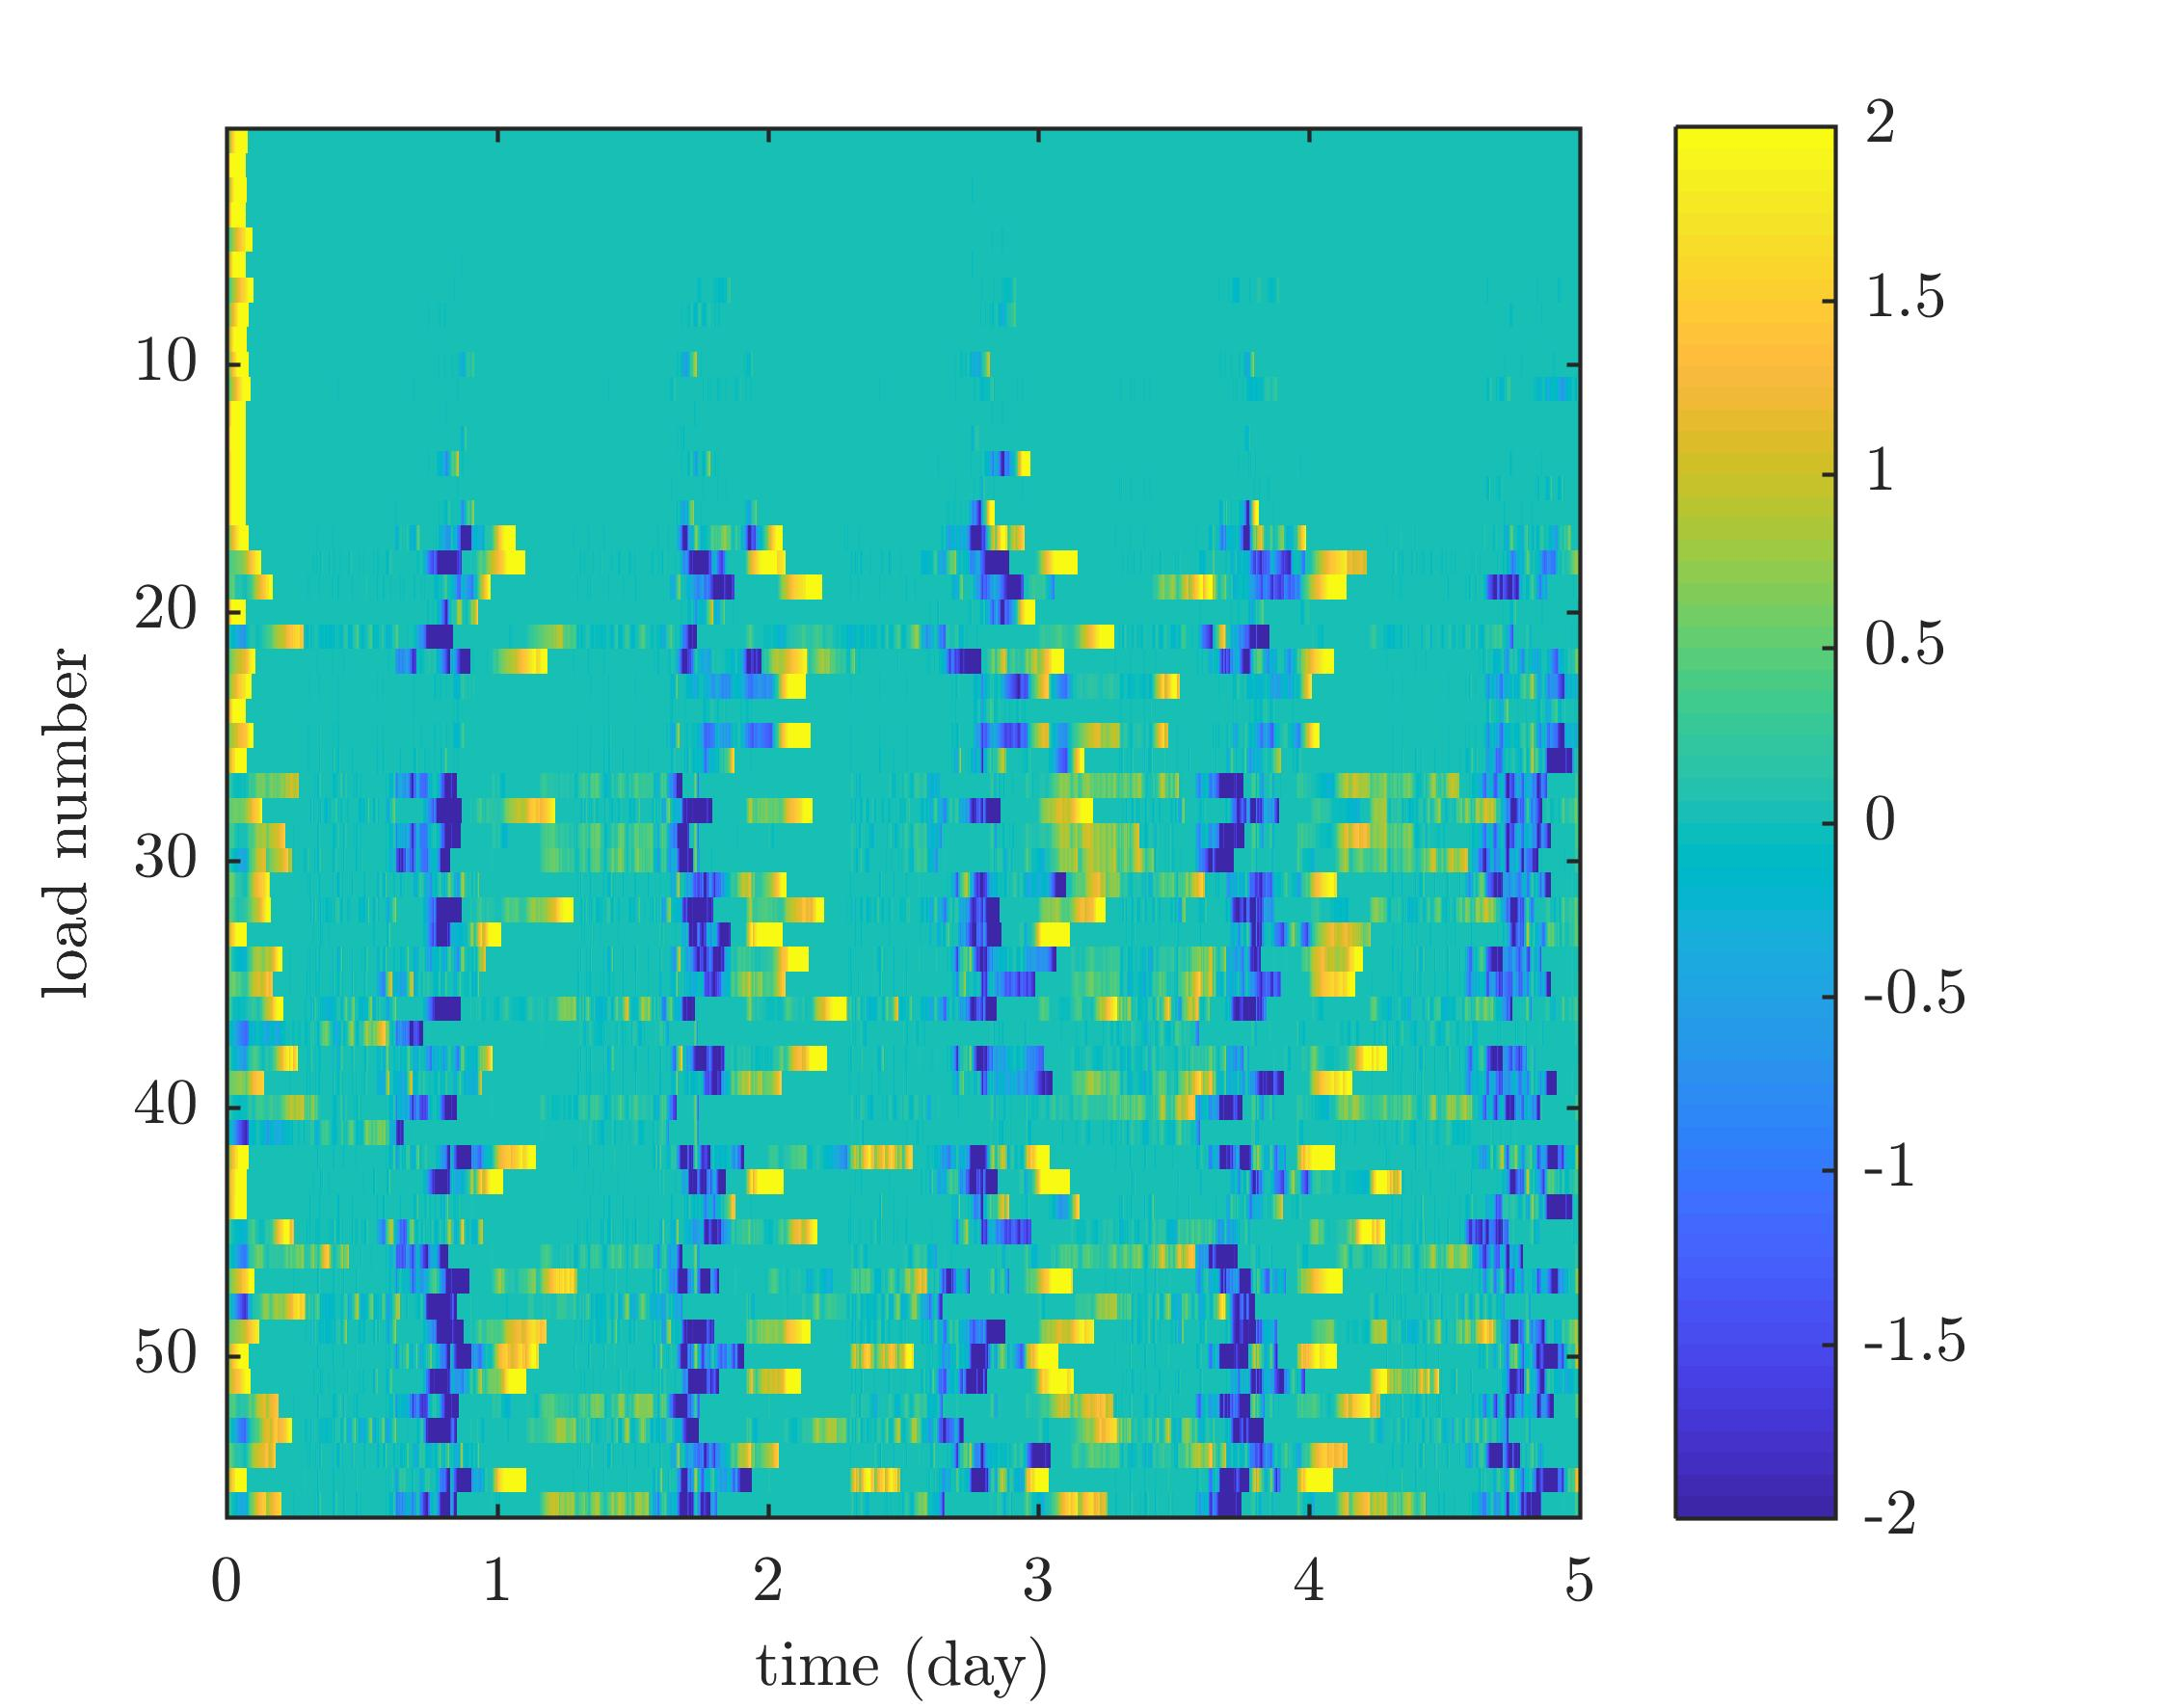
\includegraphics[width=0.5\textwidth]{_chapter4/fig/storage-aimd}
		\label{ch4:subfig:storage-aimd}
	}
	\subfloat[]{
		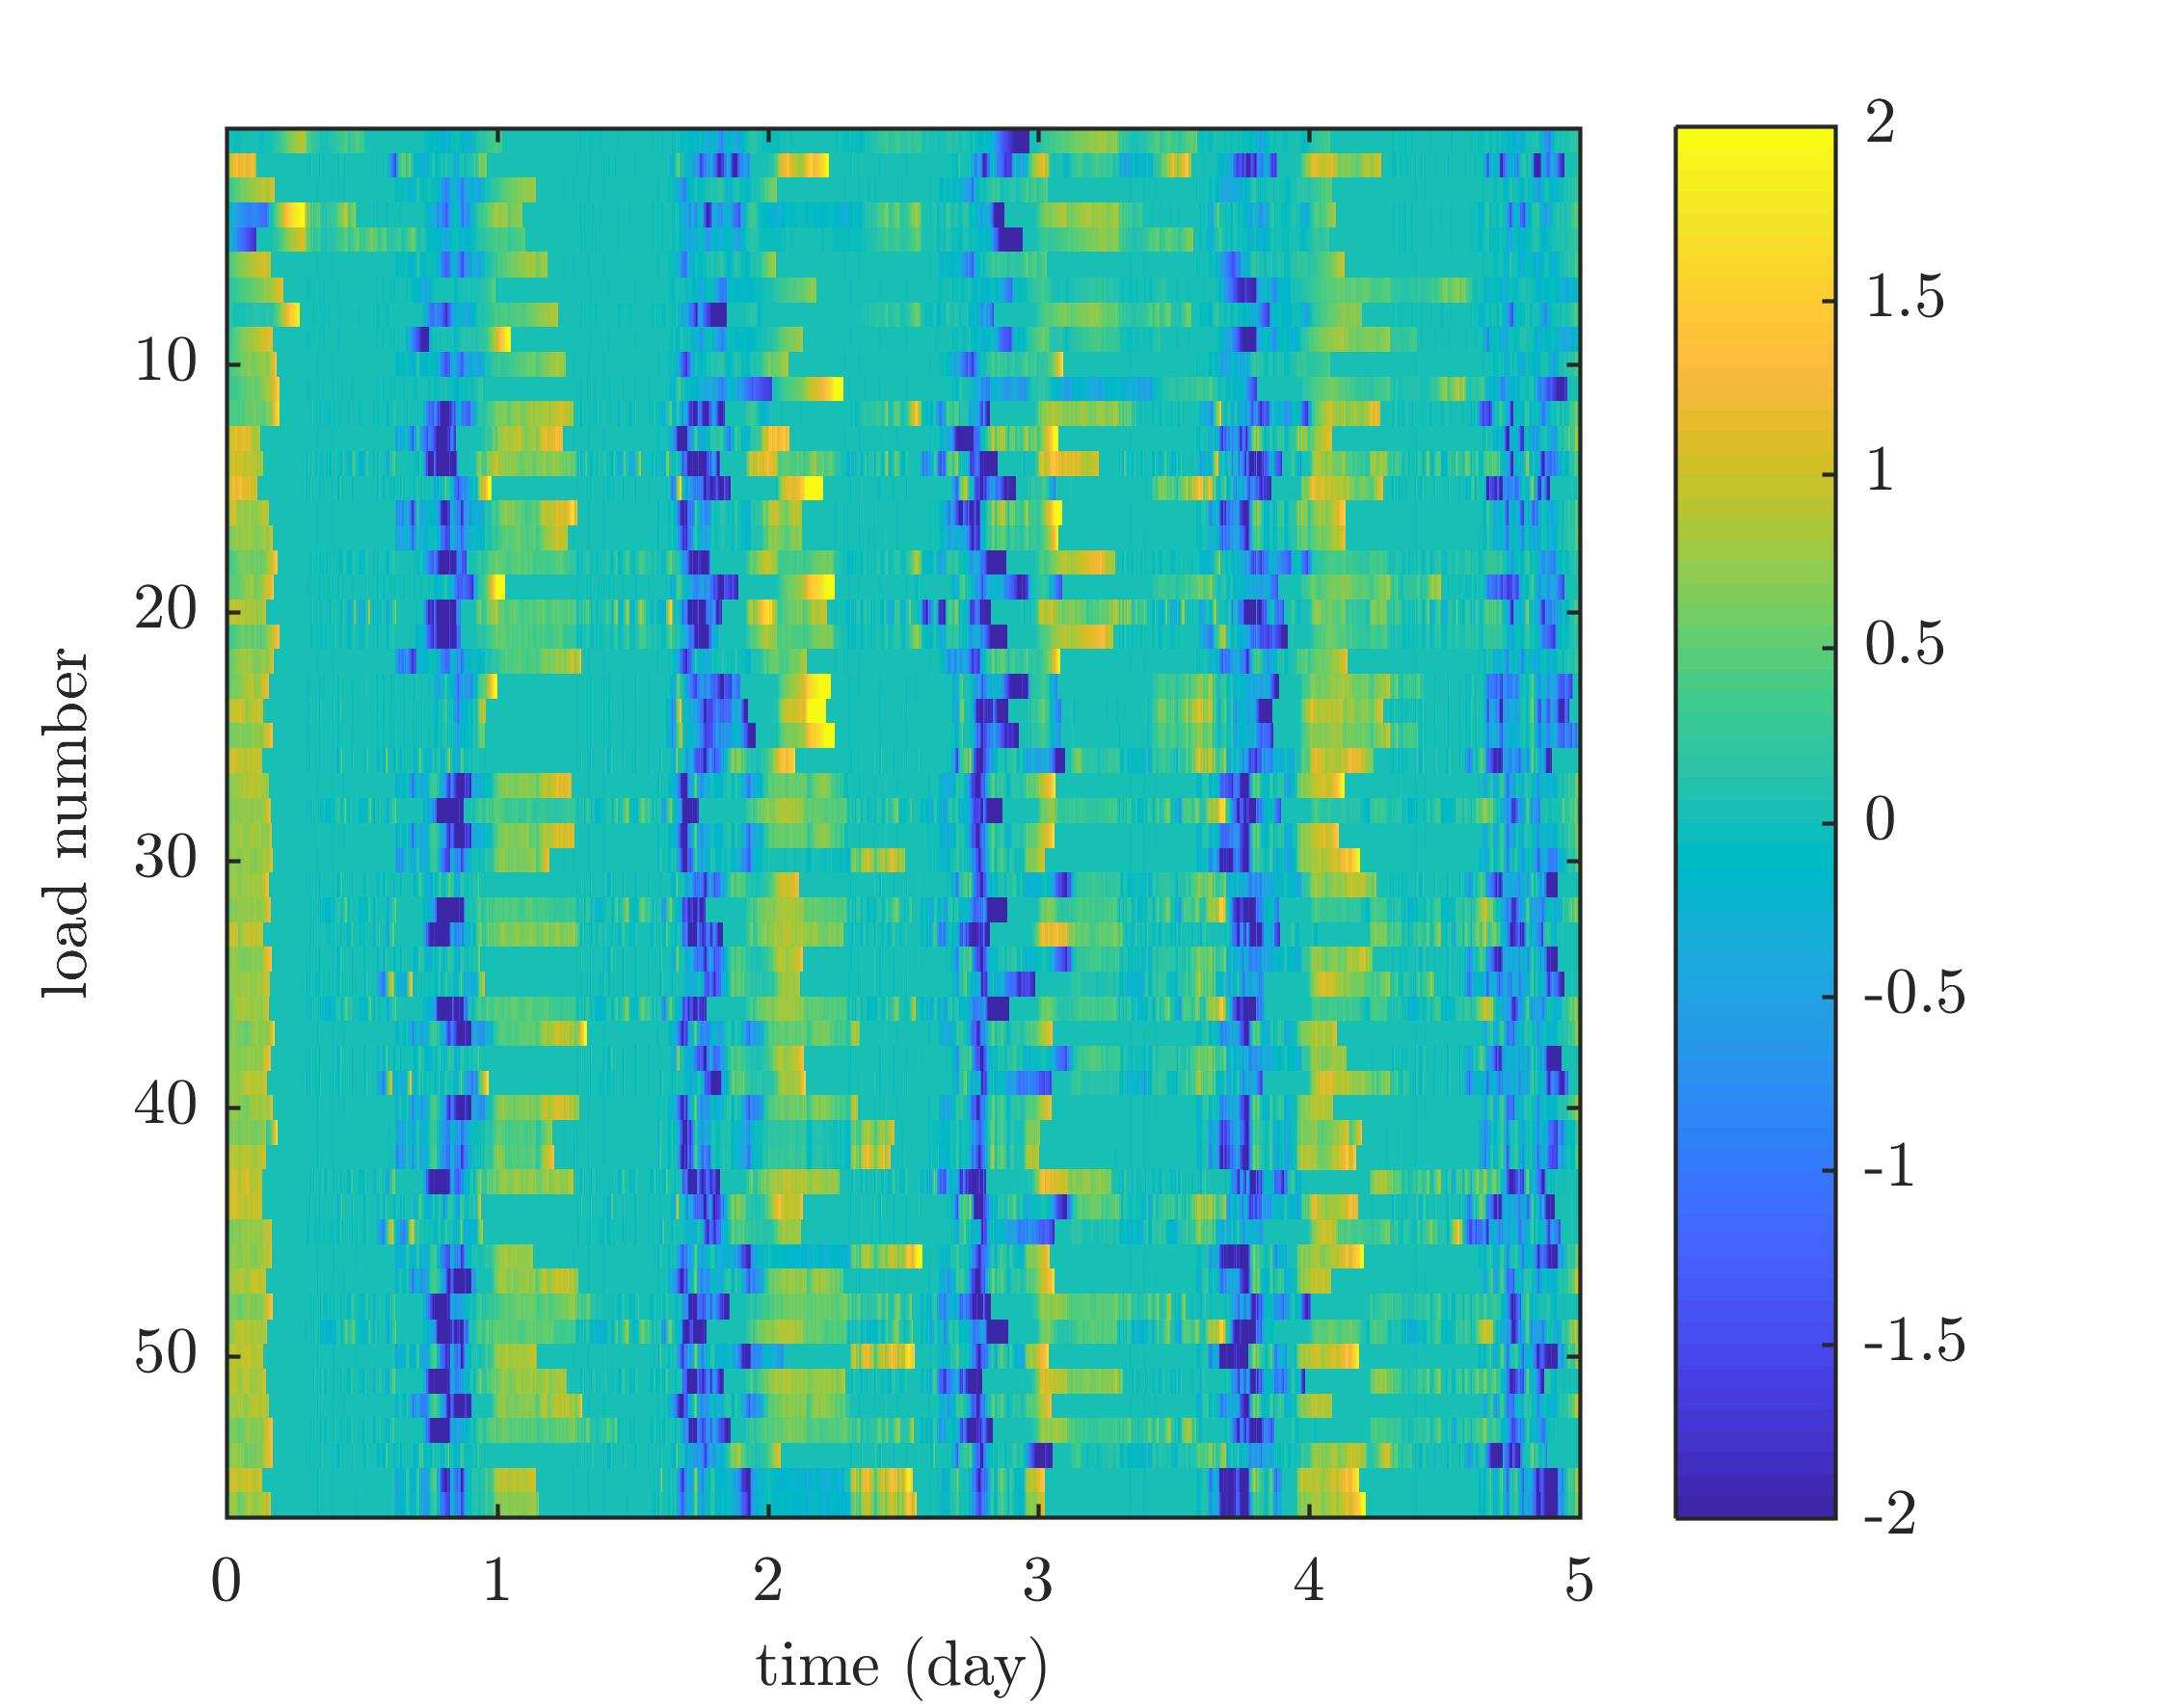
\includegraphics[width=0.5\textwidth]{_chapter4/fig/storage-aimd-plus}
		\label{ch4:subfig:storage-aimd-plus}
	}
	\caption{Battery power profiles of each load's battery storage device over four days for (a) \ref{ch4:case-c} and (b) \ref{ch4:case-d}.}
	\label{ch4:fig:storage-aimd}
\end{figure}


Figure~\ref{ch4:fig:storage-aimd} shows that only half of the deployed storage devices were active in \ref{ch4:case-c} (AIMD control), whereas all devices are utilised in \ref{ch4:case-d} (AIMD+ control).
From the recorded battery SOC profiles, the net cycling of each battery was computed and divided by the duration of the simulation to give an average daily cycling value.
This value is plotted for each load in Figure~\ref{ch4:subfig:storage-aimd-cycling-compare} - the corresponding statistical analysis is included in Figure~\ref{ch4:subfig:storage-aimd-cycling-stats}:

\begin{figure}\centering
	\subfloat[]{
		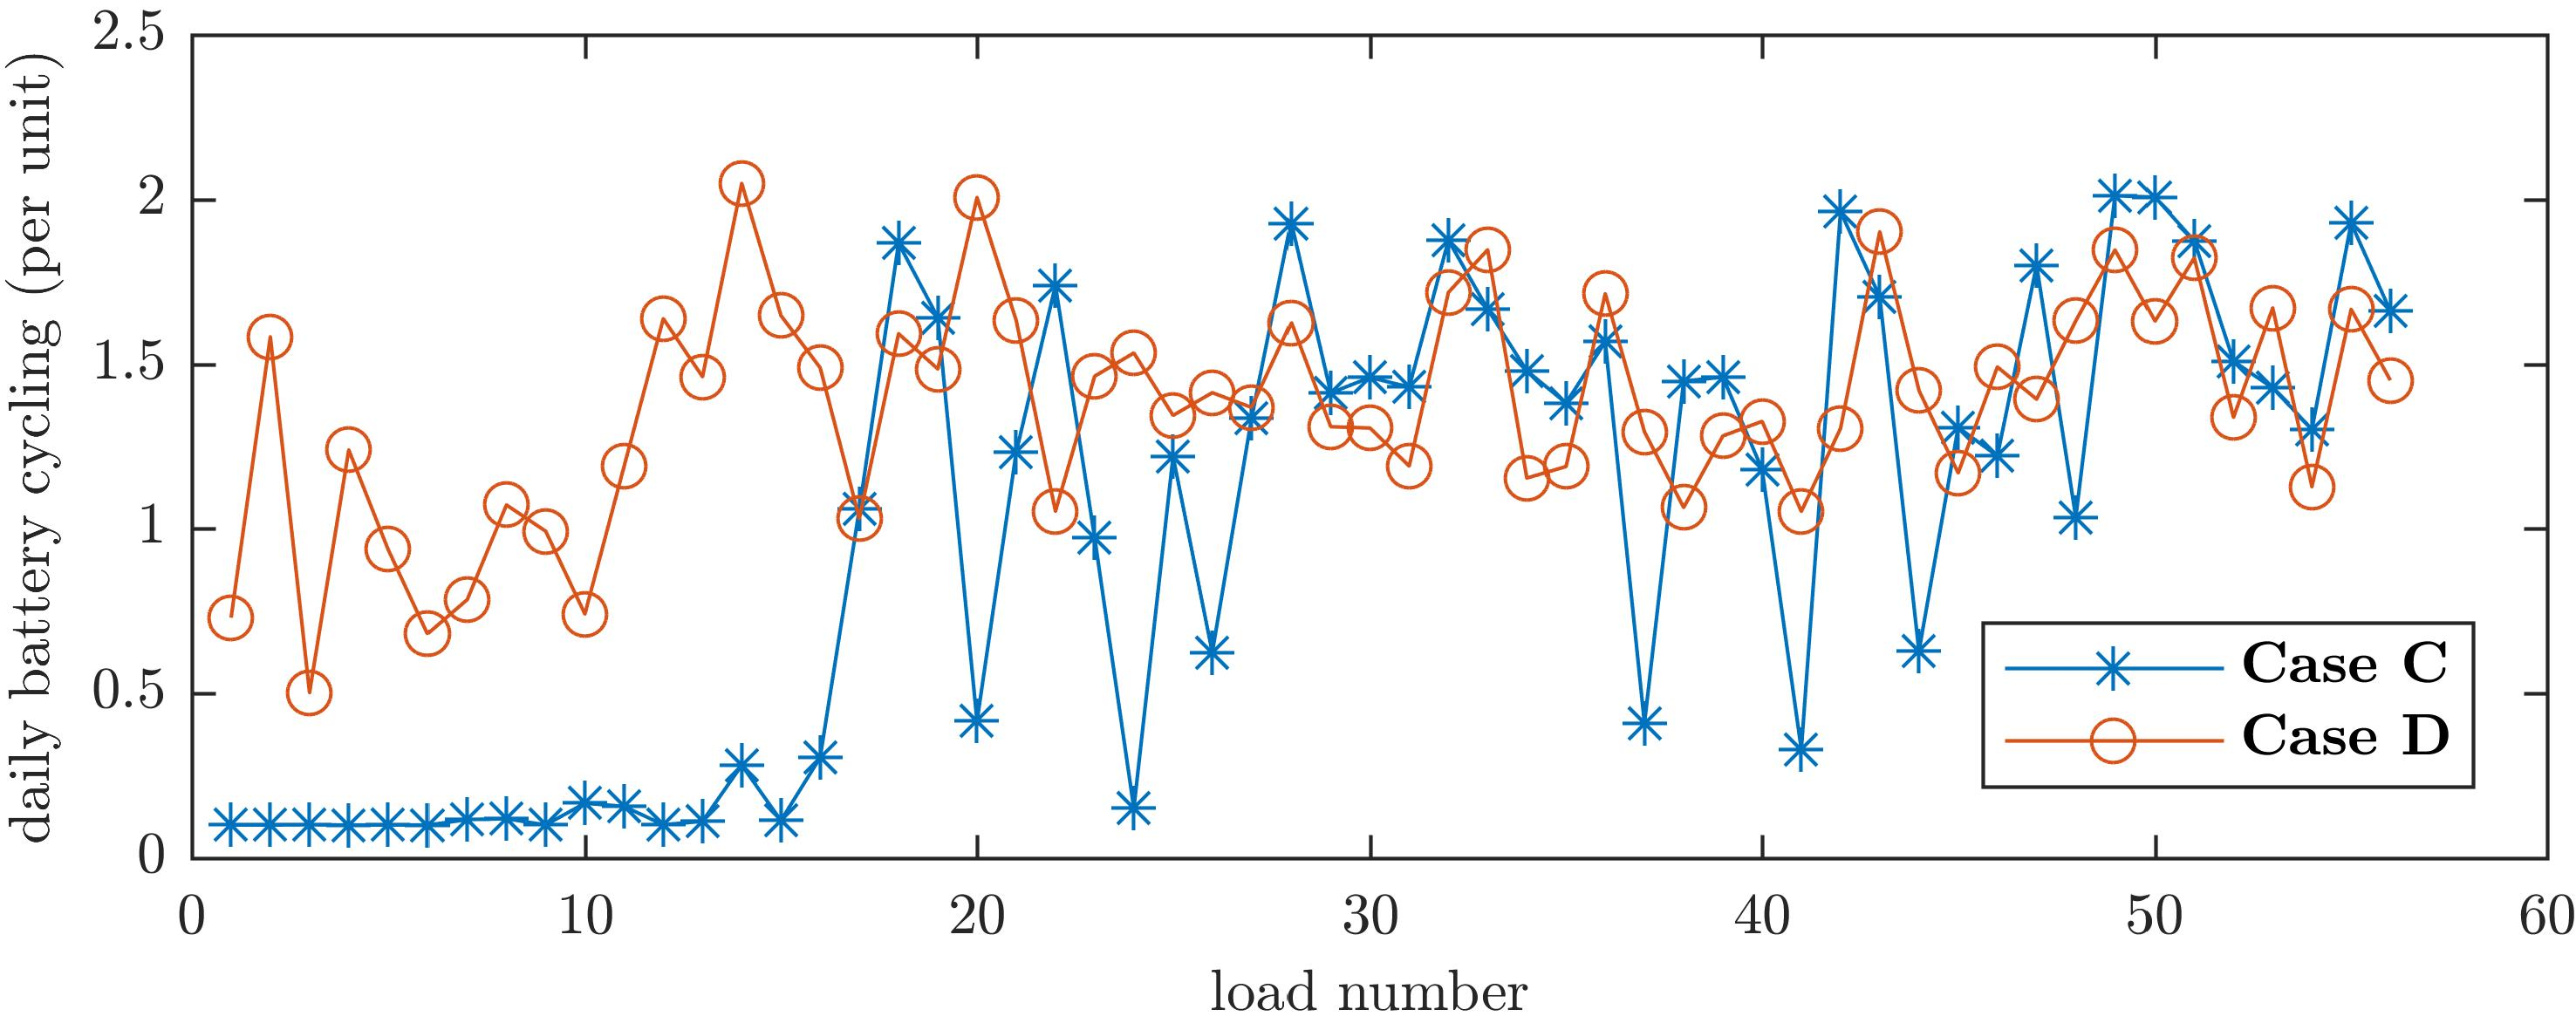
\includegraphics[height=0.3\textwidth]{_chapter4/fig/storage-aimd-compare}
		\label{ch4:subfig:storage-aimd-cycling-compare}
	}
	\subfloat[]{
		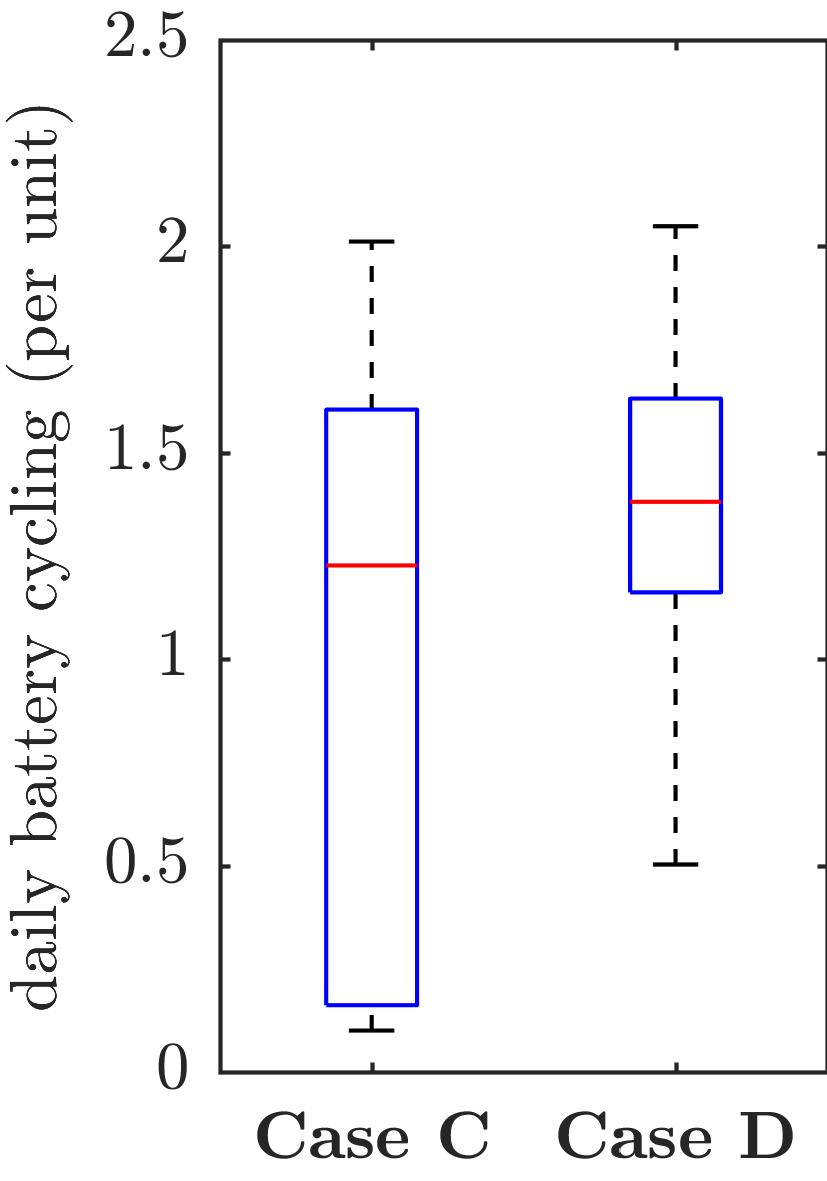
\includegraphics[height=0.3\textwidth]{_chapter4/fig/storage-aimd-compare-stats}
		\label{ch4:subfig:storage-aimd-cycling-stats}
	}
	\caption{Each load's battery cycling compared for (a) each BESS and (b) the two cases, where $\zeta_\textbf{C}^{***}=3.89$ and $\zeta_\textbf{D}^{***}=2.54$.}
	\label{ch4:fig:storage-aimd-cycling}
\end{figure}


These two plots in Figure~\ref{ch4:fig:storage-aimd-cycling} show the under-use of AIMD controlled batteries, as well as the variance in battery usage under AIMD control (\ref{ch4:case-c}) and AIMD+ control (\ref{ch4:case-d}).
In fact, when using the AIMD control, 20 out of 55 batteries experienced a battery cycling of less than 10\% per day, whereas the remaining devices were utilised fully.
This discrepancy causes the cycling performance metric of \ref{ch4:case-c} (i.e. $\zeta_\textbf{C}^{***}$) to be higher than the performance metric of \ref{ch4:case-d} (i.e $\zeta_\textbf{D}^{***}$).
Such a difference supports the assumption that AIMD+ yields a more equal battery cycling than traditional AIMD.
For a more detailed comparison however, the PARs of the batteries' daily cycling over the full range of EV and storage uptake scenarios are plotted in Figure~\ref{ch4:fig:storage-aimd-par} (Section~\ref{ch4:subsec:performance-metric-definition} gave details on all performance metrics, including $\zeta^{***}$, i.e. PAR, which is defined in Equation~\ref{ch4:equ:par-metric-c} and Equation~\ref{ch4:equ:par-metric-d}):

\begin{figure}\centering
	\subfloat[]{
		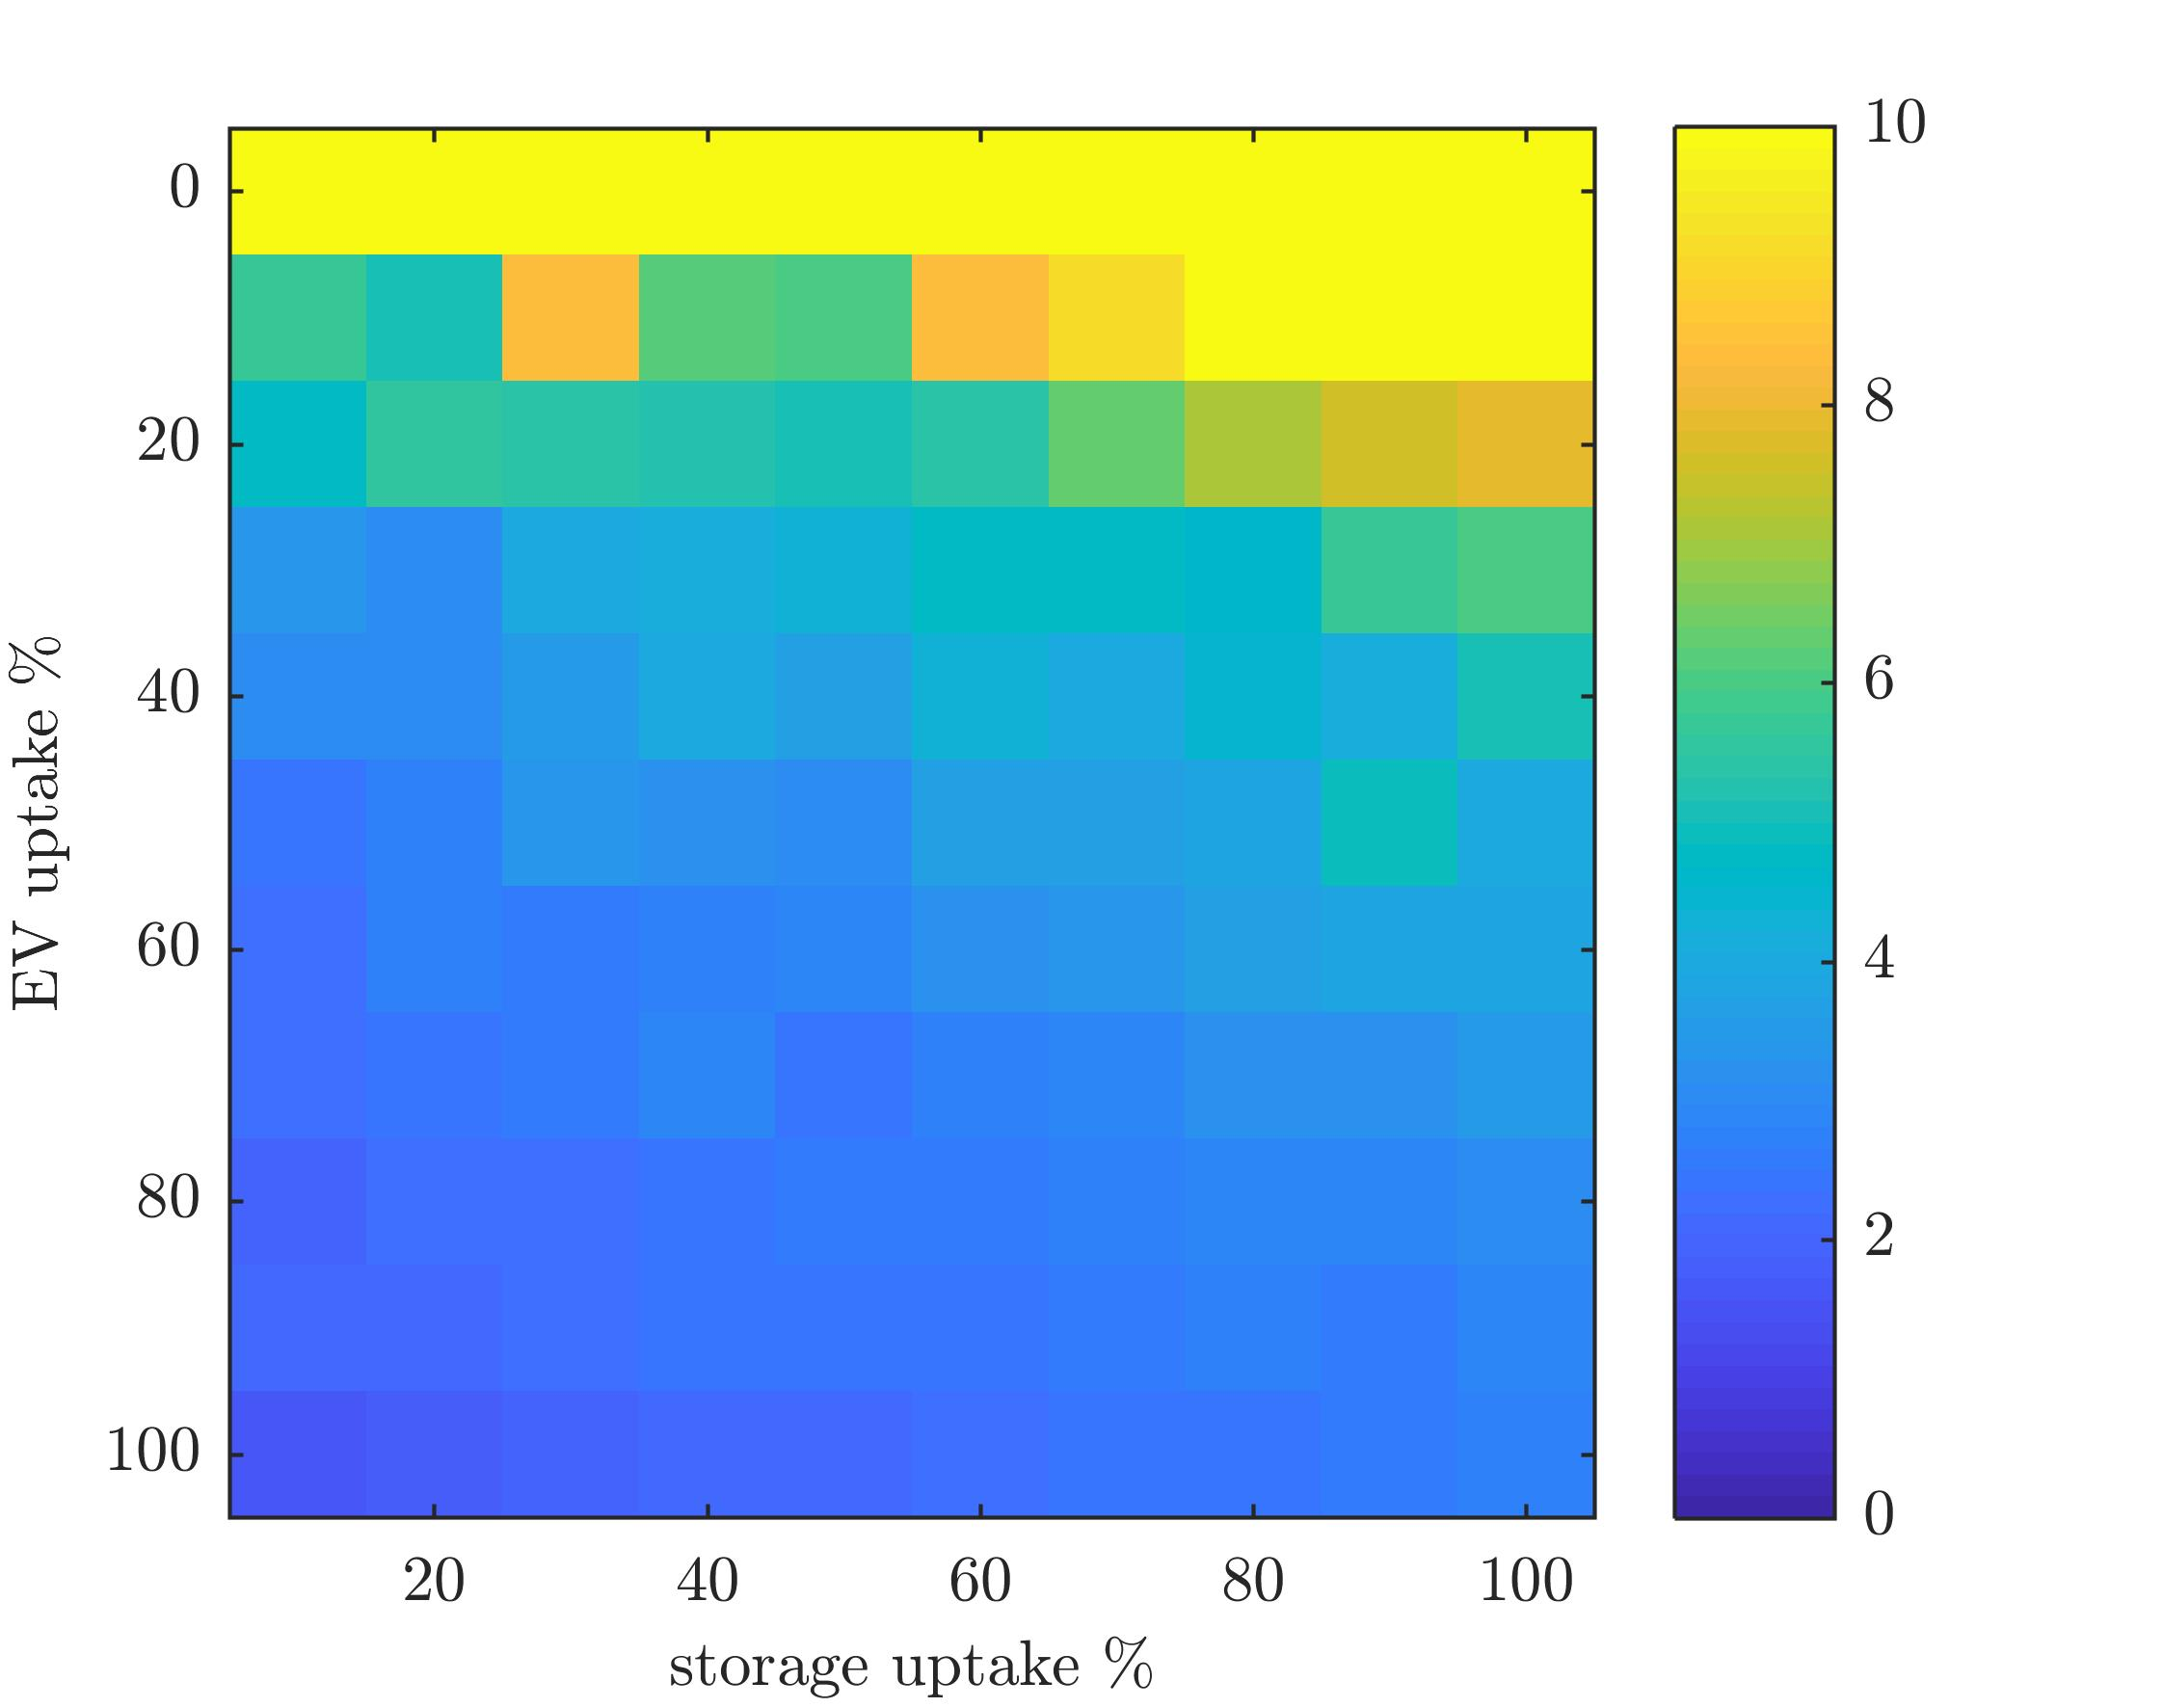
\includegraphics[width=0.5\textwidth]{_chapter4/fig/storage-aimd-par}
		\label{ch4:subfig:storage-aimd-par}
	}
	\subfloat[]{
		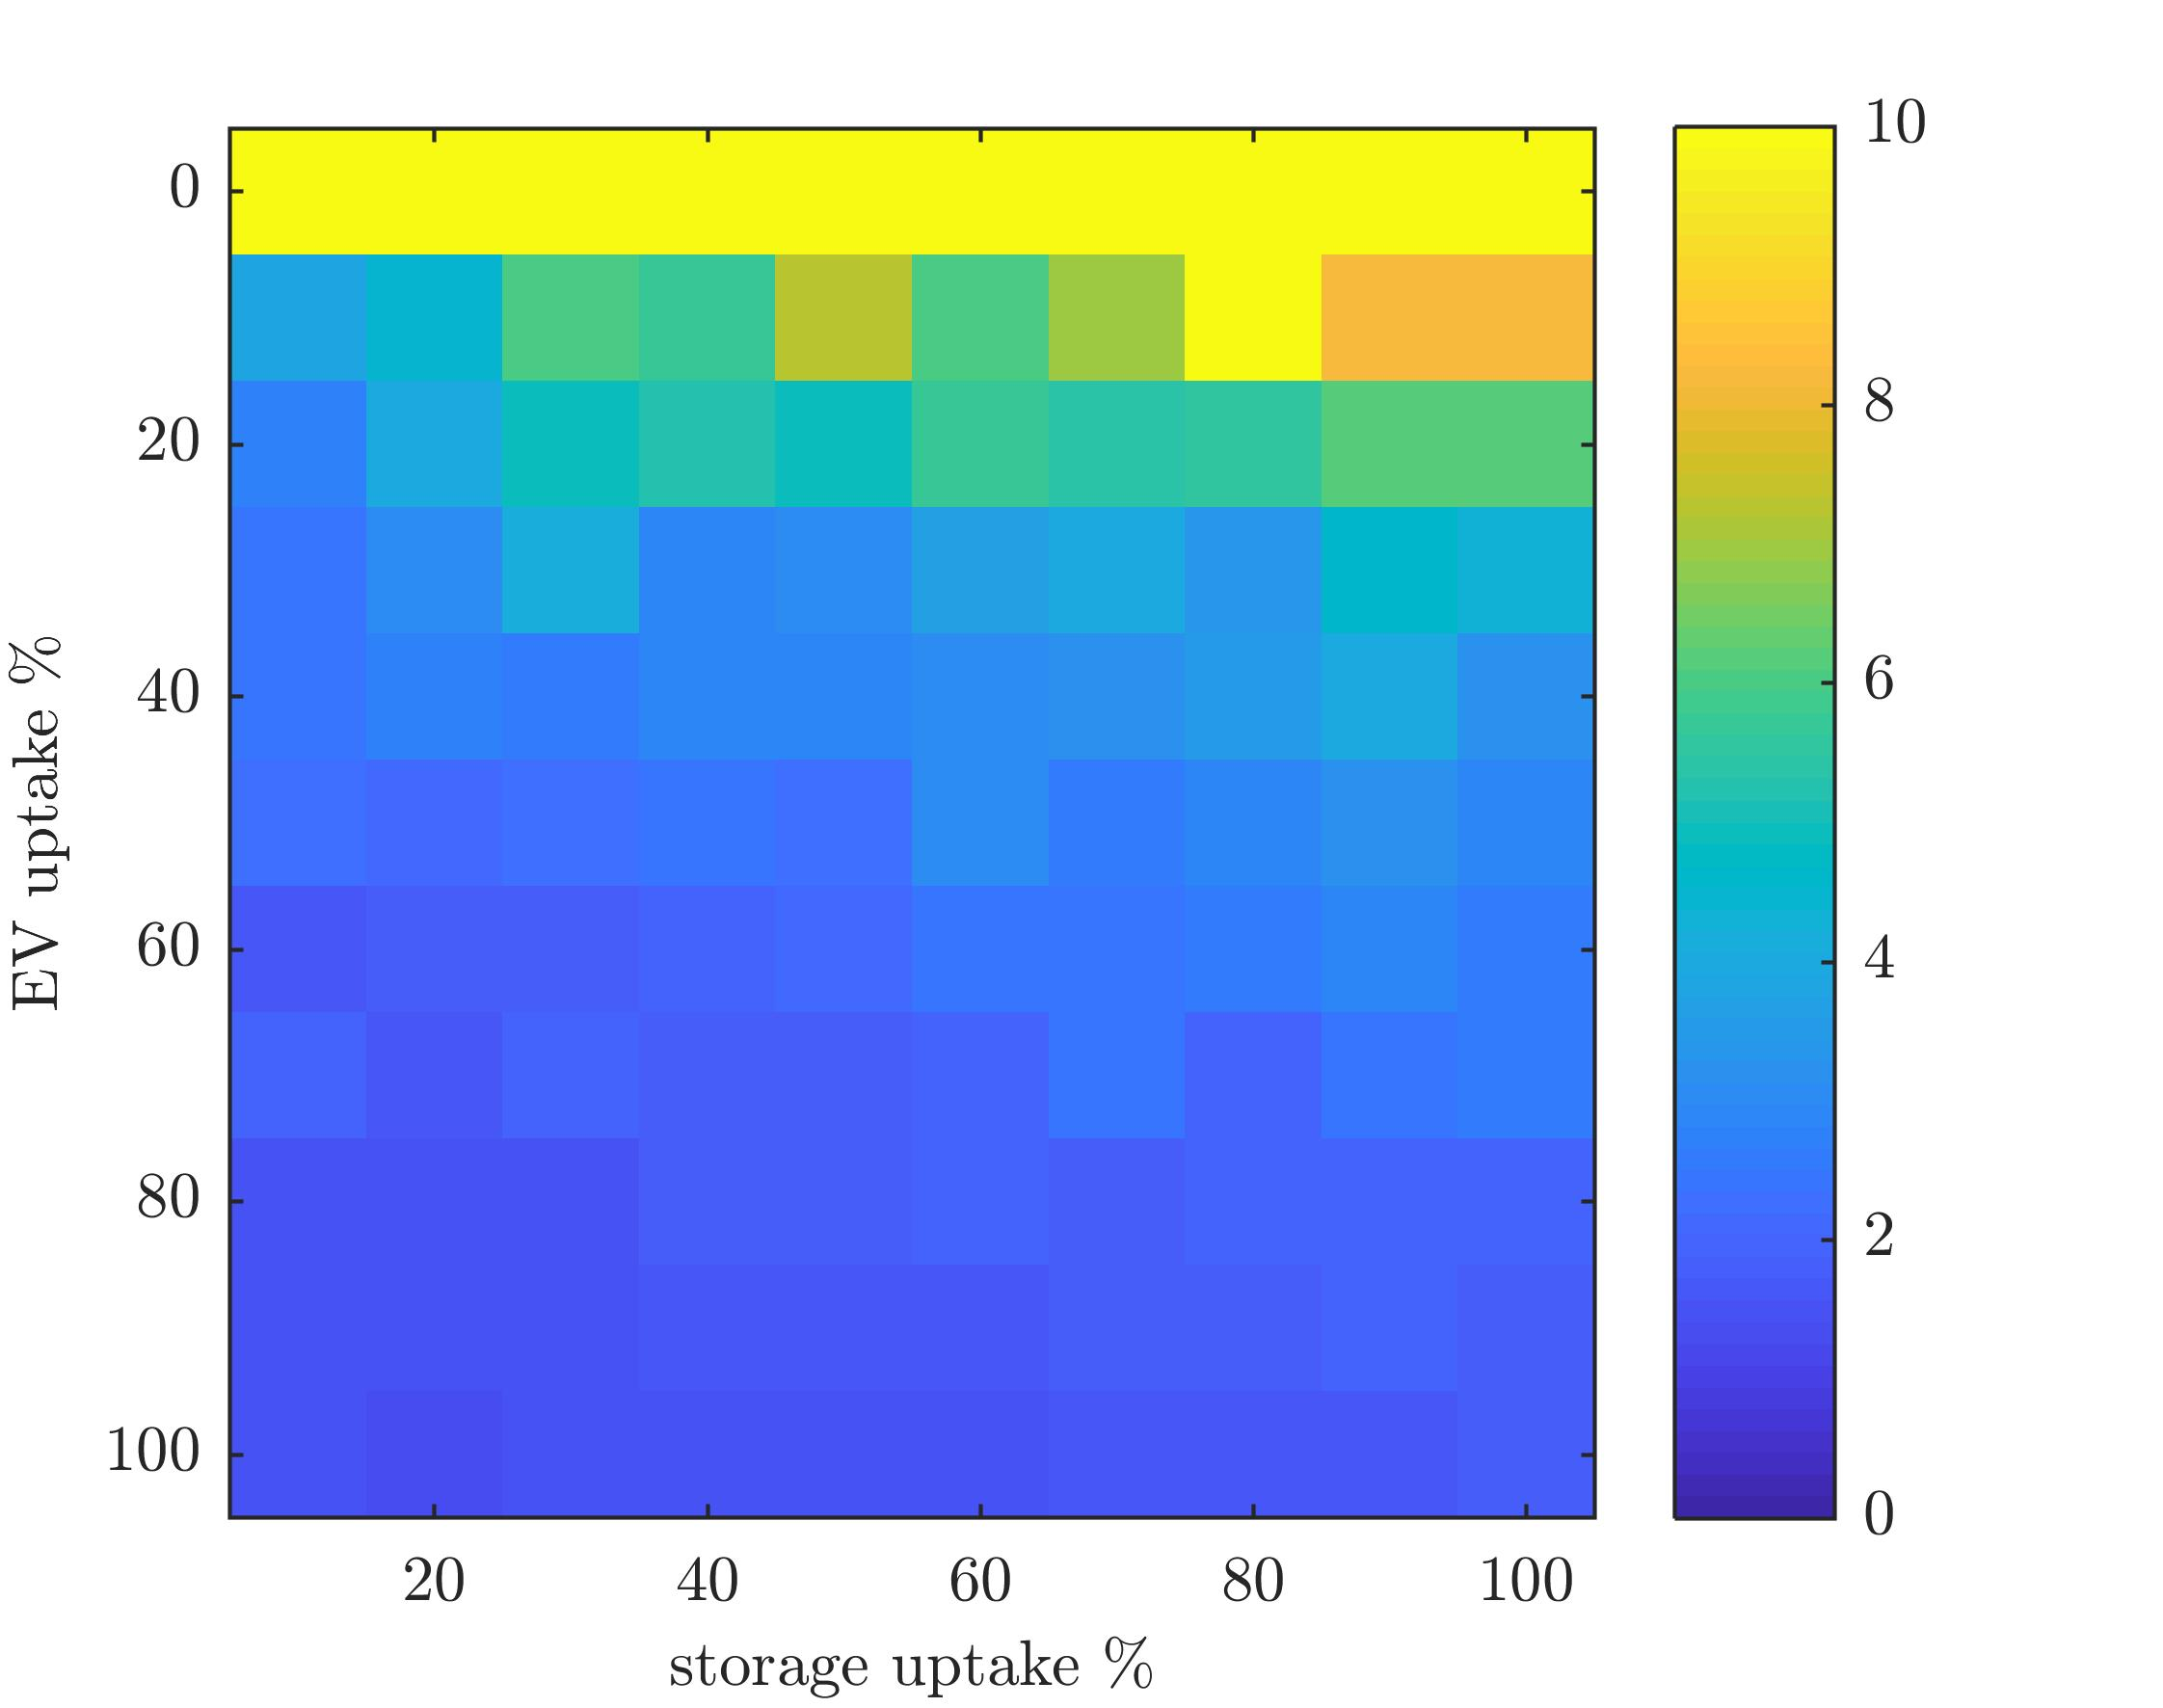
\includegraphics[width=0.5\textwidth]{_chapter4/fig/storage-aimd-plus-par}
		\label{ch4:subfig:storage-aimd-plus-par}
	}
	\caption{Peak-to-Average Ratios (PAR) of the battery cycling profiles of each load's battery storage device over four days for (a) \ref{ch4:case-c}  and  (a) \ref{ch4:case-d}.}
	\label{ch4:fig:storage-aimd-par}
\end{figure}


In Figure~\ref{ch4:fig:storage-aimd-par}, it can be seen that for any EV uptake scenario, AIMD-controlled energy storage units were cycled less equally than the AIMD+ controlled devices.
The results also show that with an increasing storage uptake, BESS were cycled less equally for both control methods.
However, AIMD+ (i.e. \ref{ch4:case-d}) always outperformed the traditional AIMD algorithm (i.e. \ref{ch4:case-c}).
When averaging the values for $\zeta^{***}$ of all batteries' SOC profiles and over all EV uptake percentages, then a clear performance difference between AIMD and AIMD+ can be observed.
These resulting averaged PARs are plotted in the subsequent figure, Figure~\ref{ch4:fig:storage-aimd-compare-par}.

\begin{figure}\centering
	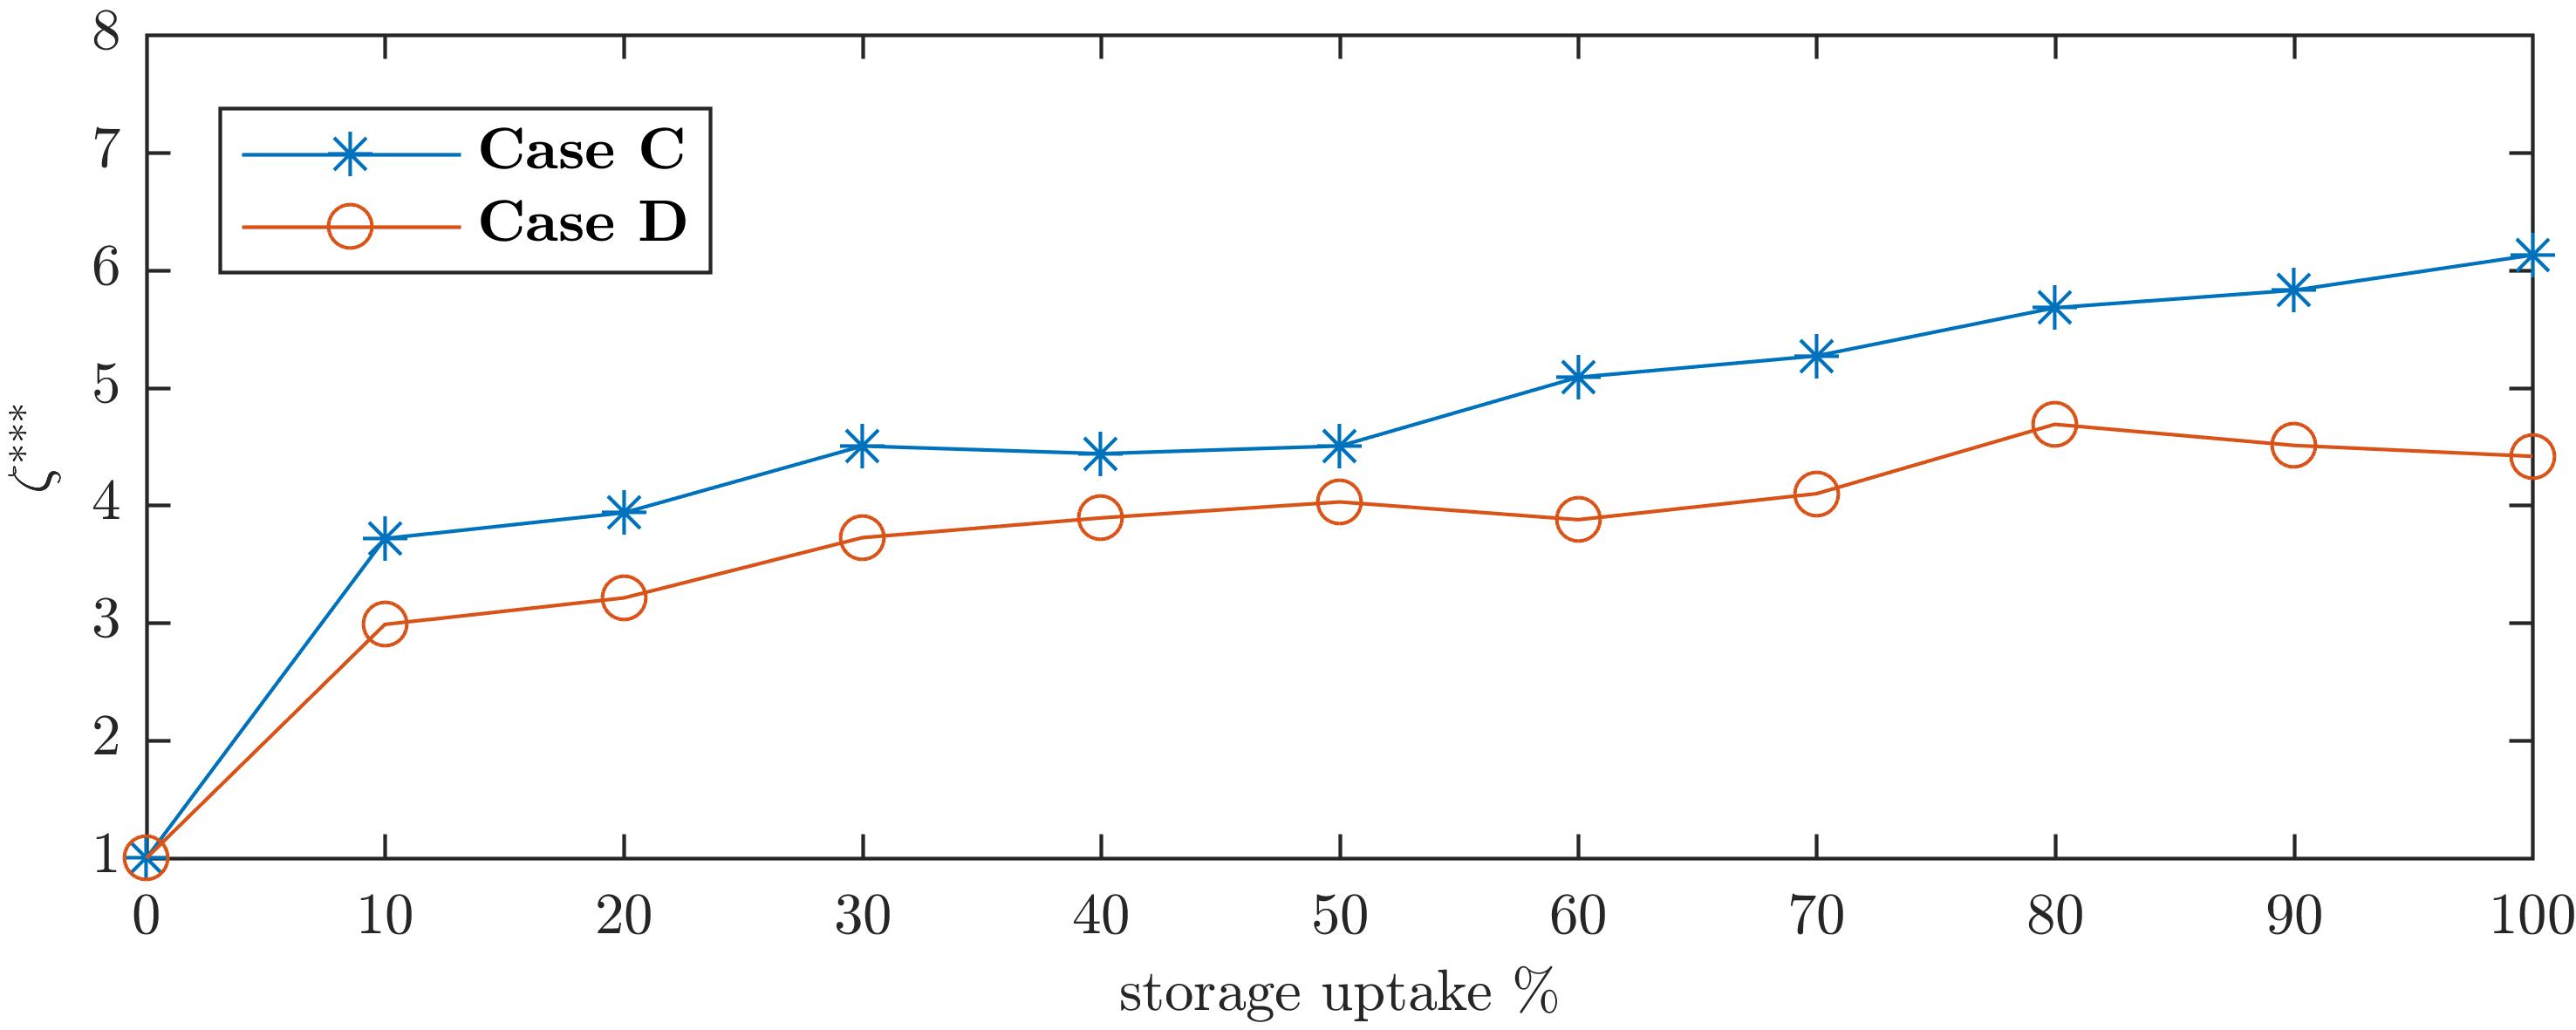
\includegraphics{_chapter4/fig/storage-aimd-compare-par}
	\caption{The performance index $\zeta_\textbf{C}^{***}$ for AIMD storage and $\zeta_\textbf{D}^{***}$ for AIMD+ storage control against storage uptake.}
	\label{ch4:fig:storage-aimd-compare-par}
\end{figure}


Although the AIMD controlled batteries were, on average, cycled less than the batteries controlled by the proposed AIMD+ algorithm, inspecting the average by itself produces a distorted understanding of the algorithm's performance.
After all, since more than half of the assigned AIMD BESS devices never partook in the network control, a lower average cycling would be expected to begin with.
The difference in cycling across all batteries, or the cycling PAR, reveals the difference between usage equality as well as effective usage.
And since a lower PAR indicates a more equal usage of the deployed batteries, AIMD+ clearly outperforms AIMD when subjected to the provided data.




